\documentclass[12pt]{article}

\usepackage{times}
\usepackage{fullpage}
\usepackage{latexsym}
\usepackage{amsmath}
%\usepackage{hyperref}
\usepackage{graphicx}
\usepackage{aclcite}
\usepackage{alltt}
\usepackage{subfig}
\usepackage{aliases}
\usepackage{multirow}

\title{Identifying Lexical Relationships and Subsitutes with Distributional Semantics}
\author{Stephen Roller\\
The University of Texas at Austin\\
{\tt roller@cs.utexas.edu}\\
\\
Doctoral Dissertation Proposal}

\date{September 7, 2016}

\begin{document}
\maketitle

\begin{abstract}
  As the field of Natural Language Processing has developed, more ambitious
  semantic tasks are starting to be addressed, such as Question Answering, and
  Recognizing Textual Entailment. Systems which approach these tasks can
  perform sophisticated inference between sentences of Natural Language, but
  often have exhibit issues of Montague-style semantics, where the meaning of
  {\em life} is {\em life$'$}. Such systems depend heavily on lexical resources
  like WordNet to provide critical information like the relationships between
  lexical items, or whether one lexical item entails another. However, lexical
  resources are expensive to create and maintain, and can never be
  comprehensive.

  Distributional Semantics has long provided a method to automatically induce
  meaning representations for lexical items from large corpora with little or
  no annotation efforts. In Distributional Semantics, words are modeled as
  vectors in high-dimensional spaces, induced by counting or modeling the
  contexts in which a word appears. The resulting representations are excellent
  as proxies of semantic similarity: words will have similar representations if
  their semantic meanings are similar. Yet, knowing two words are similar does
  not tell us their relationship, or whether one entails the other.

  In this work, we present several techniques for automatically identifying
  specific relationships or entailments from distributional representations of
  lexical semantics. Broadly, this work falls into two distinct but related
  areas: the first predicts specific taxonomic relations and entailment
  decisions between lexical items devoid of context;
  the second predicts specific lexical paraphrases in complete sentences. In
  both cases, we evaluate and emphasize generalization to novel lexical items
  which are devoid of any explicit semantic annotations.  We also provide
  analysis and insight as to how and why these models are anble to generalize
  to novel lexical items, and relate this to prior linguistic and NLP research.

  (Summary of proposed items here)
  %We propose several short- and long-term extensions to this work. In the
  %out-of-context models, we propose applying our model to a broader group of
  %lexical relations, and including additional useful features in
  %classification.  In the in-context work, we propose extensions which improve
  %handling of very rare context items, analyzing the relationships between
  %paraphrases. In the long-term, we propose stronger models of in-context
  %representations, and unifying the out-of-context and in-context models in
  %one of several possible ways.
\end{abstract}

%\pagebreak
\tableofcontents
\pagebreak

\section{Introduction}

As the field of Natural Language Processing (NLP) has developed, significant
progress has been made in many areas of research, especially those in ``lower''
levels of the Bernard Vauquois's famed Triangle, like Part-of-Speech tagging
\cite{toutanova:2003:naacl} and Parsing \cite{chen:2014:emnlp}.  Significant progress
has also been made even in some very difficult semantics tasks,
like Named Entity Recognition \cite{needcite}, Sentiment Analysis
\cite{socher:2013:nips} and Document Classification \cite{zhang:2016:naacl},
and Coreference Resolution \cite{durrett:2013:emnlp}.

Today, there is great deal of emphasis on sophisticated semantics
tasks that require inference and synthesis of knowledge. These include tasks
like Question Answering (QA), where computers must read and answer questions
about passages \cite{hermann:2015:nips,needcite}, and Recognizing Textual
Entailment (RTE), where computers must decide whether a hypothesis utterance
logically follows from a given text
\cite{marelli:2014:semeval,bowman:2015:emnlp,beltagy:2016:cl}.

Much progress has been made in systems which perform these sort of sophisticated
logical inferences, especially as common benchmarks and datasets have started
to become common \cite{marelli:2014:semeval,bowman:2015:emnlp}. Yet these
systems ultimately must work over individual lexical items to form a
conclusion, and require knowledge about the relationships between lexical
items. Consider the following example:
\footnote{Mention ``Montague's curse'', as I like to call it?}
\begin{quote}
  Text: The bright girl reads a book.\\
  Hypothesis: The smart child looks at pages of text.
\end{quote}
Any language processing system wishing to infer the second sentence from
the first must know quite a bit of world knowledge: it must know that
girl is a kind of child, and that bright and smart are synonyms in this
context; that books contain pages of text, and that reading involves looking
at some text.

Although significant progress has been made on the text of
Rich Textual Entailment, many of these systems ultimately depend on some lexical
resources
\cite{beltagy:2014:semeval,bjerva:2014:semeval,lai:2014:semeval,marelli:2014:semeval,beltagy:2016:cl}.
The most famous lexical resource is WordNet \cite{miller:1995:acm}, which organizes the lexicon into a
large ontology containing many thousands of annotations of relationships
between different lexical items, though many other resources also exist
and are used \cite{baker:1998:acl,baroni:2011:gems,baroni:2012:eacl,ganitkevitch:2013:naacl,jurgens:2012:semeval,levy:2014:conll,turney:2015:nle}.
Unfortunately,
resources as thorough as WordNet are extremely expensive and intensive to
create, and since language is ever-changing, they are inevitably always
incomplete. As such, dependence on manually constructed resources represents one weak point in some Natural Language Understanding
systems. Even modern Neural Network approaches, which attempt to learn
entailments without explicitly depending on these resources, cannot make
entailment predictions about words which were not in the training data
\cite{bowman:2015:emnlp,cheng:2016:arxiv}.

Distributional Semantics offers a potential solution to these issues of lexical
coverage. Distributional Semantics takes inspiration from the famous quote,
``You shall know a word by the company it keeps'' \cite{firth:1957:la}. In
Distributional Semantics, representations of word meaning are automatically
induced by counting or modeling the {\em contexts} in which a word appears.
Distributional Semantics is often sometimes called Vector Space Models (VSM) of
language, as words are represented as vectors a high-dimensional vector space.
Words with similar semantics will have similar vectors in this induced
geometric space. Since VSMs do not require annotated corpora, they are used and
studied as an alternative or predictor of particular lexical resources \cite{needcite}.

In this work, we approach the question as to whether Distributional Semantics
can be leveraged to predict some of the lexical inferences necessary in tasks
like RTE. Namely, we present techniques and models for predicting specific
lexical relationships, entailments, and subsitutions using Distributional
Semantics. In Lexical Relationship detection and Entailment detection, we must
predict whether two words exhibit specific relationships, like hypernymy (is-a
relationships) or meronymy (has-a relationships). We present two original
models which can learn to predict hypernymy and sometimes other relations,
and characterize their performance on different datasets, relations. We also
present an original model for Lexical Substitution, in which we must predict a
context-specific synonym for a given target word; we argue that Lexical
Substitution is a form of lexical entailment in context.

Finally, we propose several extensions to this completed work. In the
short-term, we propose drawing a stronger connection between Lexical
Substitution and lexical relationships, analyzing the sort of lexical
relationships which we can and cannot predict in our model. We propose
extending our Lexical Substitution model to better handle out-of-vocabulary
(OoV) issues for very rare context items. We also propose further analysis of
our Lexical Relationship models to see if additional relationships can be
automatically predicted, and consider whether the model can do all-words
relationship prediction.  In the long-term, we wish to consider whether our
Lexical Substitution model can be improved by removing or alleviating a strong
independence assumption in the previous model, and how the Lexical Substitution
and Relationship Detection models could be potentially unified.


\section{Background and Related Work}

\subsection{Textual Entailment}

\subsection{Distributional Semantics}
Distributional Semantics is a powerful tool for automatically inducing semantic
representations for lexical items \cite{turney:2010:jair,erk:2012:llc}.  The
core notion is that of the {\em Distributional Hypothesis}, that if two words
appear in similar {\em contexts}, they can be assumed to have similar meaning.
This idea has a long history in the semantics and philosophical literature that
can be traced back over 60 years
\cite{wittgenstein:1953:pi,harris:1954:word,firth:1957:la}. In its modern form,
Distributional Semantics involves finding {\em vector space} representations of
words which are constructed by counting or modeling the contexts in which a
particular word appears. According to the Distributional Hypothesis then, words
with similar vectors can be assumed to have similar meanings
\cite{turney:2010:jair}.

\begin{figure}
\centering
\begin{minipage}{7cm}
\begin{scriptsize}
\begin{alltt}
         the furry {dog} is friendly to
and manipulate the {dog} 's lips and
       as a clever {dog} ; two to
a reputation among {dog} trainers of having
    also among the {dog} breeds most likely
 the very earliest {dog} shows and kennel
        as a guard {dog} and to hunt
   the mechanic 's {dog} began to howl
\end{alltt}
\end{scriptsize}
\end{minipage}\qquad
\begin{minipage}{3cm}
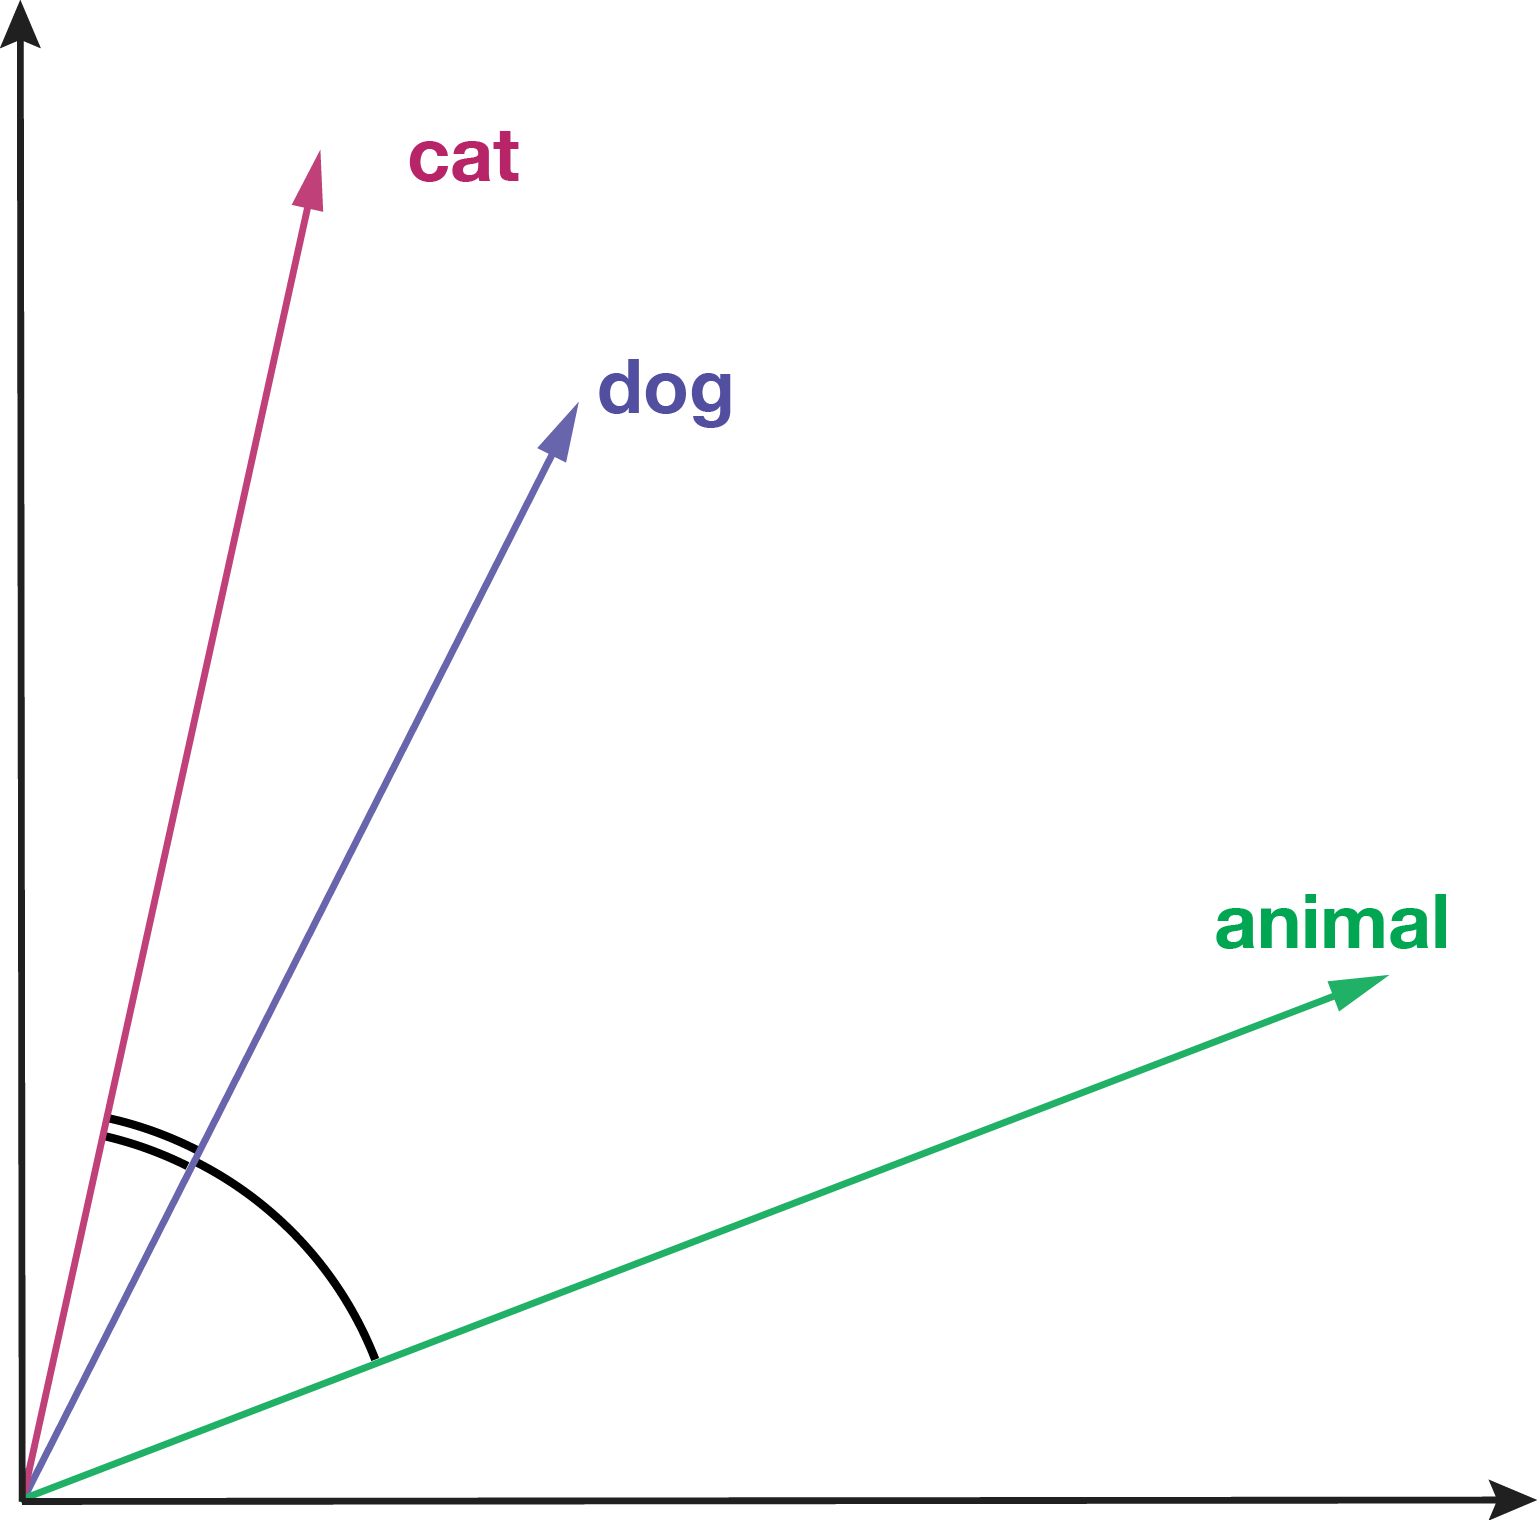
\includegraphics[width=3cm]{figures/vsm}
\end{minipage}
\caption{Contexts of the word {\em dog}, and cartoon drawing
of word vectors.}
\label{fig:vsm}
\end{figure}

In its simplest form, vectors are induced by defining a vector space where
each dimension in the space corresponds to a particular context word. A large,
unannotated corpus of text is then iterated, finding instances of a given word,
like {\em dog}, and incrementing a count for each of the word's {\em
co-occurrences}, or words appearing to the left or right of the target word
{\em dog}, as in Figure~\ref{fig:vsm}. With a large enough corpus, coherent
statistical patterns begin to form. For example, the word {\em furry} is likely
to be used to describe both {\em cat} and {\em dog}, which is then reflected in
the vector counts. After constructing vector representations for the words {\em
cat} and {\em dog}, we can then compare these vectors using {\em cosine
similarity}:
\begin{equation*}
  \text{cosine}(u, v) = \frac{\sum_i u_iv_i}{\sqrt{\sum_i u_i^2 \sum_i v_i^2}}
\end{equation*}
Here, $i$ iterates over all the different context dimensions, like {\em furry}
or {\em kennel}, and cosine similarity is defined over the range of $[0, 1]$.
Words with similar vectors will have a small angle between them, and therefore
a high cosine similarity (e.g. close to 1).

In practice, usually the distributional vectors are more sophisticated in their
construction than raw co-occurrence counts. Typically, words and contexts below
a certain threshold are omitted from the co-occurrence matrix, as extremely
rare words have few counts and therefore impoverished representations. The
co-occurrence matrix is also usually transformed using some non-linearity;
one common choice is Positive Pointwise Mutual Information (PPMI), where the
raw co-occurence count between a word $w$ and context $c$ is transformed,
\begin{equation*}
  \text{PPMI}(w, c) = \max\left(0, \log\frac{P(w, c)}{P(w)P(c)}\right)
\end{equation*}
Pointwise Mutual Information measures roughly how many times more likely
do these two items co-occur more than chance, while Positive PMI additionally
co-occurrences which occur less often than chance. Different transformations,
like Mutual Information, conditional probability, and softplus, are also
sometimes seen in the literature, and each emphasizes different forms of
similarity.

Another important aspect of Distributional Semantics is how context is defined.
In the example of Figure~\ref{fig:vsm}, we showed that context can be defined
as three words to the left and right of the target word, but there are
alternatives. For example, using very large windows of similarity results in
emphasizing more topical similarity, e.g. doctor and hospital, while smaller
windows emphasize more functional similarity, e.g. doctor and surgeon
\cite{needcite,levy:2014:acl}.

Context can be also defined as {\em syntactic neighbors} extracted
from a dependency parse \cite{pado:2007:cl}. For example, in Figure~\ref{fig:syn},
the contexts for the word {\em chased} would be {\em nsubj+dog} and {\em
dobj+tail}. Distributional Spaces defined in this manner tend to emphasize
the {\em selectional preferences} of words, or the tendency of certain
relations to occur with certain arguments.

\begin{figure}
  \centering
  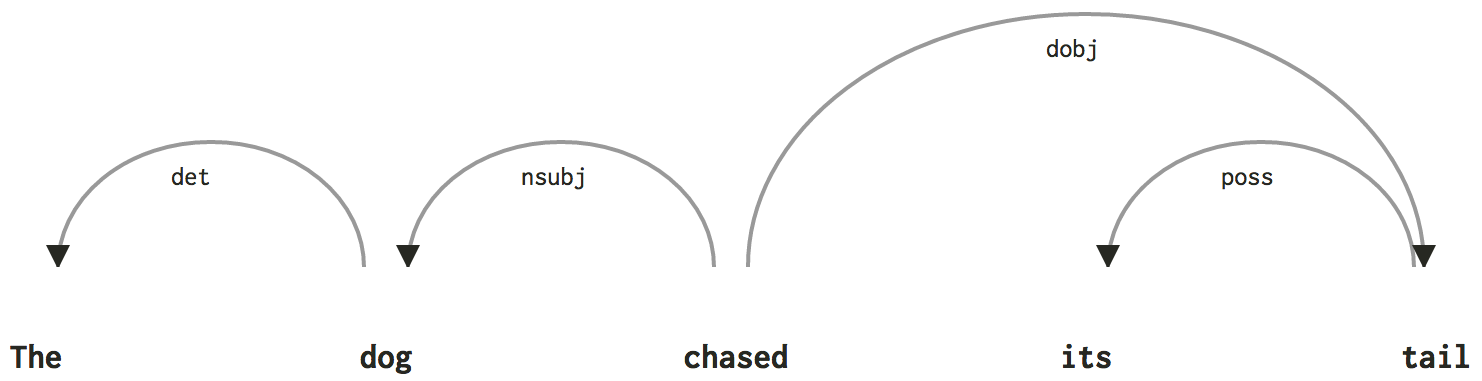
\includegraphics[width=0.75\textwidth]{figures/syn}
\caption{Example of a dependency parse for ``The dog chased its tail.'' In
a syntactic distributional space, contexts are defined as adjacent nodes
with their labeled edges.}
\label{fig:syn}
\end{figure}

One final notion in Distributional Semantics we wish to review is that of
dimensionality reduction. As described earlier, the distributional vector
spaces are very high-dimensional; bag-of-words spaces have many thousands of
dimensions (or sometimes as large as the entire vocab, e.g.
\newcite{pennington:2014:emnlp}, while syntactic spaces often have a millions,
e.g. \newcite{baroni:2010:cl}. Efficiently dealing
with these large, extremely sparse vectors can sometime be troublesome, so
we often opt to use some form of {\em dimensionality reduction}, like
Singular Value Decomposition (SVD) \cite{landauer:1997:pr} or Nonnegative Matrix
Factorization (NNMF) \cite{lee:2000:nips}. In dimensionality
reduction, the co-occurrence matrix $M$ is typically assumed to be factorizable
into two lower-rank matrices,
\begin{equation*}
  M = VC^{\top}
\end{equation*}
where $V$ is some lower dimension representation of word vectors, and $C$
is the corresponding lower dimension representation of the context items.
Interestingly, the recent, popular Word2Vec algorithm \cite{mikolov:2013:iclr}
can also be viewed as a form of dimensionality reduction \cite{levy:2014:nips}.

\subsection{Lexical Entailment}

It can be difficult to give an exact definition of Lexical Entailment, but in
this document we define it as any lexical relationship where a typical,
cooperative reader would logically assume a given consequent from a given
antecedent.\footnote{Katrin, help please!  can you think of something better
with a citation I can use?} This includes many classical lexical relations,
like hypernymy (a girl {\em is a} child; a dog {\em is an} animal), and
meronomy (a girl {\em has} eyes; a dog {has a} tail), but also many
nonclassical ones too. For example, a {\em dissertation} implies a {\em
committee}, but the exact relationship between these items would be difficult
to pigeonhole into a category, or generalize to other items.

There has been a great deal of research around predicting lexical entailment
automatically from text; we cannot possibly enumerate all the work on this
problem done in all of NLP, but we aim to cover some influential approaches,
and emphasize attempts to do this with distributional semantics.

One important, early work in this task was that of Hearst patterns
\cite{hearst:1992:coling}, which are specific textual patterns highly
indicative of particular relationships. Common Hearst patterns include
phrases like ``X such as Y,'' ``X including Y,'' which are both highly
indicative of hypernymy; and possessives, like ``X's Y'', can be indicative
of meronomy. In fact, the previous sentence contains several Hearst patterns
{\em about} Hearst patterns. Later, the Hearst pattern method by
\newcite{snow:2004:nips} to include a variety of syntactic patterns rather than
pure textual patterns. By using syntactic parses, some longer distance patterns
are more easily captured, like ``X such as Y and Z'', which can be more
trivially transformed to ``X such as Z'' in a syntactic parse.

In another vein of research, others have proposed how
hypernymy relationships might be viewed holistically in corpora.
One lasting hypothesis has been the Distributional Inclusion Hypothesis (DIH)
\cite{zhitomirsky-geffet:2005:acl}, which states that the contexts in which a
hypernym appears should be a superset of all its hyponyms, or subordinate
words. Though this seems to be strictly false\footnote{Consider {\em \#The
animal barked loudly at its bowl of animal food.}}, a considerable amount of
work has assumed it to be at least partially true, including our own.

Early work in identify lexical entailments using distributional spaces was
focused mostly on attempts to find unsupervised similarity measures to identify
specific relationships from the word vectors
\cite{weeds:2004:coling,clarke:2009:gems,kotlerman:2010:nle,lenci:2012:starsem,santus:2013:thesis}.
The reasoning went that, with perhaps the right corpus, the right
distributional space, and the right similarity measure, perhaps hypernym pairs,
or at least candidate pairs, could be readily identified using only word
vectors vectors. This view was further highlighted by the fact that the
ubiquitious cosine similarity tends to highlight co-hyponym pairs more than
other relations \cite{baroni:2011:gems}. Many of the proposed measures were
based on the Distributional Inclusion Hypothesis in one form or another
\cite{clarke:2009:gems}, or a hybrid of DIH and cosine similarity
\cite{kotlerman:2010:nle,lenci:2012:starsem}.

Increasingly, it became obvious that unsupervised measures did not work
as well as the community hoped, the community began working
on entailment detection as a supervised task. \newcite{baroni:2012:eacl}
proposed, as a preliminary baseline of a novel dataset, training a simple
baseline classifier to predict whether word pairs were either hypernyms or
nonhypernyms. Although they reported accuracies in the high 90s, others later
realized this was due to issues of {\em lexical memorization}, or a special
kind of overfitting
\cite{roller:2014:coling,weeds:2014:coling,levy:2015:naacl}. As such, more
recent works have emphasized their performance when {\em individual words are
held out entire}, so that the same word can never appear in both training and
testing sets \cite{roller:2014:coling,kruszewski:2015:tacl,levy:2015:naacl}.
We discuss more about this issue of Lexical Memorization in
Section~\ref{sec:lexmem}.

\subsection{Lexical Substitution}
\label{sec:lexsub}

While the Lexical Entailment task described above is mostly about predicting
fixed, global relationships between words, Lexical Substitution is about
finding specific paraphrases for words {\em in a given sentential context}.
That is, we wish to also consider how polysemy can change the sort of
lexical entailments derived by a system.

Consider again our example from the introduction: while the previous section
aims to understand that a {\em girl is-a child}, it does not attempt to find a
relationship between {\em bright} and {\em smart}. This is because the word
{\em bright} has multiple meanings, and there needs to be some sort of
reasoning in order to consider that the appropriate synonym of {\em bright}
is {\em smart} in this context, but not {\em luminous} or {\em colorful}.
More formally, in Lexical Substitution, we wish to identify what
words could replace a given target word in a particular sentence, while
perserving the meaning of the whole sentence. Evaluation is typically
performed by comparing a system's predictions to actual substitutes generated
by humans asked to perform the same task.

In the original SemEval 2007 version of the Lexical Substitution Task, systems
were required to generate up to ten potential substitutes for the given target
word and context, and not given any additional information. As such, early
Lexical Substitution systems relied heavily on lexical resources like WordNet
to obtain a list of {\em candidate substitutes}. Then, using various custom
features, they would extract features and learn to rank substitutes for their
appropriateness \cite{mccarthy:2007:semeval}. Later, researchers began noting
the difference between candidate generation and candidate ranking, and then
focused research on mostly the ranking task \cite{needcite}. The vast majority
of these systems are based on the notions of finding substitutes based on {\em
Selectional Restrictions} and {\em Selectional Preferences}, or
limitations/preferences about the types of arguments and modifiers words tend
to take \cite{needcite}.

Today, many have begun returning to the generation-and-ranking task
\cite{melamud:2015:naacl,kawakami:2016:iclr,roller:2016:naacl,melaumud:2016:conll},
but opting to avoid lexical resources like WordNet.  Curiously, to date, the
best performing systems in Lexical Substitution are ones which are unsupervised
with respect to the task: either they are trained for some auxiliary task like
Machine Translation \cite{kawakami:2016:iclr}, or they are similarity methods
over distributional models \cite{roller:2016:naacl} or language modeling
\cite{melamud:2015:naacl}. This could be because of a lack of recent effort in
directly supervised versions of the task \cite{szarvas:2013:naacl}, or because
lexical substitution datasets are relatively small compared to the size of the
corpora used in machine translation and distributional semantics.

\section{Completed work}

\subsection{Asym Model for Lexical Entailment (Roller et al., 2014)}
\label{sec:asym}

Most baseline similarity measures in distributional semantics, like cosine,
have the unfortunate property that they're symmetric: $\text{cosine}(a, b) =
\text{cosine}(b, a)$. While this necessary to obey the Triangle Inequality, it
is a fatal flaw in any application involving lexical entailment: although {\em
girl} implies {\em child}, but the opposite does not hold. As such, trying to
predict lexical entailment based solely using symmetric measures will always
fail.

This has been recognized widely in the
literature for some time, and numerous asymmetric, unsupervised similarity measures have been
proposed
\cite{weeds:2003:emnlp,zhitomirsky-geffet:2005:acl,clarke:2009:gems,kotlerman:2010:nle,santus:2013:thesis},
mostly inspired by the Distributional Inclusion Hypothesis. However, their
performance tend to be lackluster \cite{clarke:2009:gems} or brittle
\cite{kotlerman:2010:nle}. This lead to the question: are the measures just
overly sensitive to noise in distributional vectors, or is the Distributional
Inclusion Hypothesis fundamentally flawed? If the unsupervised are measures
are simply too sensitive to noise, perhaps using supervised techniques can
improve performance.  To this end, we propose Asym, a simple supervised model
that is inherent asymmetric \cite{roller:2014:coling}. 

At its core, the model is inspired by the famous result of
\newcite{mikolov:2013:iclr}, who observed that vector subtraction can be used
to perform some kinds of analogical reasoning in some kinds of distributional
spaces: e.g., ${\tt king} - {\tt man} + {\tt woman} \approx {\tt queen}$.
Interestingly, this vector subtraction approach reasonably models many
grammatical relationships (singular/plural, verb conjugations) and some limited
semantic relationships (gender, capital/country). Asym exploits this
behavior for the task of hypernymy and lexical relationship prediction.


The Asym model is a simple model which uses the {\em vector difference} between
the hypothesized hypernym and hyponym as input features to an off-the-shelf
classifier. For example, given a distributional vector for {\tt animal} and
a vector for {\tt cat}, we use the vector ${\tt animal} - {\tt cat}$ as the
features for a positive example, while the vectors for
${\tt cat} - {\tt animal}$ and ${\tt animal} - {\tt sofa}$ are inputted
as negative examples. Additionally, we also give the {\em element-wise squared
difference vector} as features to the classifier. That is, for a given hypernym, hyponym
pair of words $(H, w)$, we compute the final feature space defined as:
\begin{align*}
  A_i(H, w) & = H_i - w_i\\
  B_i(H, w) & = (H_i - w_i)^2\\
  \text{features}(H, w) & = \langle A; B\rangle,
\end{align*}
where $\langle A; B\rangle$ is the vector {\em concatenation}. This computation
is performed for all examples in our dataset, and then the features$(H, w)$
vector and the classification label are used to train a Logistic Regression
classifier.

One significant advantage of this model over the prior work is its direct
connection to the Distributional Inclusion Hypothesis: since our model uses the
vector difference as input, it naturally measures whether $a_i$ is
greater than $c_i$, effectively acting as a strict-subset measurement. The
element-wise-squared part of the input features measures whether they have a
large absolute difference, effectively caputring ``equal'' part of the
``less than or equal'' relation. As such, the model describes a form of {\em
Selective Distributional Inclusion Hypothesis}, which presupposes that the DIH
holds, but only for particularly relevant dimensions.

To evaluate our model, we train and measure accuracy of the Asym model on
two datasets in a variation of leave-one-out cross validation (LOOCV) and
measuring absolute accuracy. In this variation of LOOCV, we selected one word
from the vocabulary in the datasets, and considered {\em all pairs} with that
word to be test pairs. The remainder of word pairs, which did not contain the
held out word, are treated as training pairs. This prevent classifiers from
memorizing that words like {\em animal} are simply more likely to be hypernyms.

Since different types of distributional spaces exhibit different properties
\cite{pado:2007:cl}, we evaluate our model on two distributional
spaces which use a simple Bag-of-Words context.  The {\em Window-2 BoW} space
counts content words two words to the left and right of targets as contexts,
while the {\em Sentence BoW} space counts all content words within complete
sentence bounadries. Both spaces are reduced to 300 dimensions using the
Singular Value Decomposition \cite{landauer:1997:pr}.

We evaluate our model on two datasets. The first, {\bf LEDS}
\cite{baroni:2012:eacl}, contains 1385 hyponym-hypernym pairs as positive
examples and 1385 negative pairs which were generated by randomly shuffling the
positive examples. As such the model only contains hypernymy and random
relations, and we train a binary classifier. The second dataset is {\bf
BLESS} \cite{baroni:2011:gems}, which contains annotations of word relations
for 200 unambiguous, concrete nouns from 17 broad categories. Each noun is
annotated with its co-hyponyms, meronyms, hypernym and some random words.
Since there were four relations, we trained four one-vs-all classifiers, and
predicted the relation with the highest score; in this way, the model
can learns to detect three different lexical relations, though this
was not our primary research interest at the time.

We compare our model with two baselines: the first is a random baseline,
which just guesses randomly for the balanced LEDS dataset, and always
the most common class ({\em no-relation}) for BLESS. We also compare to the
model proposed in \newcite{baroni:2011:gems}, which uses the {\em concatenation}
of the $H$ and $w$ vectors and trains an off-the-shelf polynomial Support
Vector Machine \cite{needcite}.

\begin{table}
  \centering
  \begin{tabular}{|lc|cc|}
    \hline
    {\bf Classifier} & {\bf Space} & {\bf LEDS.} & {\bf BLESS.}\\
    \hline
    Random Baseline              &   -      & .50          & .46      \\
    \hline
    \newcite{baroni:2011:gems}   & Window 2 & .81          & .76      \\
    \newcite{roller:2014:coling} & Window 2 & {\bf .85}    & {\bf .84}\\
    \newcite{baroni:2011:gems}   & Sentence & .78          & .73      \\
    \newcite{roller:2014:coling} & Sentence & .82          & .80      \\
    \hline
  \end{tabular}
  \caption{Accuracy of {\svm} and {\logreg} on {\bless} and {\entailment}
  using different spaces for feature generation. Performance is measured as
  the average accuracy across all folds of the leave-one-out cross validation
  experiment.}
  \label{tab:asymresults}
\end{table}

Table~\ref{tab:asymresults} shows the results for our initial experiment.
First we notice that both models strongly outperform the random baselines,
indicating there is some successful learning in the models. We also see that
the Window 2 space performs better than the Sentence space in all four
comparisons, indicating it is likely the task depends more heavily {\em
functional} properties of words than {\em topical} properties of words. We will
see further evidence of this in Section~\ref{sec:hfeatures}.

Finally, we see that the Asym model outperforms the model proposed by
\newcite{baroni:2011:gems} in all four comparisons, indicating something about
our feature architecture is superior to mere concatenation. Interestingly,
in unreported experiments, we found that dropping the square-difference terms
severely hurt the performance of our model, emphasizing these features
immense importance. We will discuss more of why these features are so
important in Section~\ref{sec:lexmem}. Incidentally, at the same time that
\newcite{roller:2014:coling} was published, \newcite{weeds:2014:coling} and
\newcite{fu:2014:acl} also proposed supervised hypernymy models based on
{\em vector difference}, but neither of these employ the square-difference
terms.

We also test our interpretation of Asym as measuring a form of {\em Selective}
Distributional Inclusion. After training the model's parameters on the BLESS
dataset, we compare the model's learned hyperplane to the {\em context
vectors} obtained in the Singular Value Decomposition. We then select the 500
features most similar to the model's hyperplane, and then extract a
distributional space limited to only these context items. If our Selective
Distributional Inclusion Hypothesis is true, we would expect these 500
dimensions to highly compliment existing similarity measures based on the
Distributional Inclusion Hypothesis. A careful reader should note this is
necessary, but {\em not} sufficient to show the model obeys the SDIH, as we are
effectively comparing unsupervised models with supervised ones.

We measure every word pair's similarity using three similarity measures:
cosine, Clarke, and invCL. Cosine similarity acts as our control, and
should not change substantially between the
original and selective distributional spaces, while the others, which are
based on Distributional Inclusion, should. The second similarity measure,
{\em Clarke}, measures roughly what percentage of the hyponyms' mass is contained
within the hypernym \cite{clarke:2009:gems}:
\begin{equation*}
  \text{Clarke}(H, w) = \frac{\sum_i \min(H_i, w_i)}{\sum_i H_i};
\end{equation*}
The final similarity measure, {\em invCL}, extends Clarke to additionally
measure what percentage of the hypernym's mass is {\em not} contained within
the hyponym \cite{lenci:2012:starsem}, extending Clarke to roughly measure
{\em strict} containment:
\begin{equation*}
  \text{invCL}(H, w) = \sqrt{\text{Clarke}(H, w)(1 - \text{Clarke}(w, H))}.
\end{equation*}

We compute all three similarity measures across all the word pairs in BLESS,
and computed Mean Average Precision (MAP) across all pairs for each measure
and distributional space. Ideally, we should see that, compared to the original
space, the selective distributional space has higher Clarke and invCL values
for hypernyms, and lower Clarke and invCL values for the other relations.
Table~\ref{tab:mapscores} shows the results of this experiment.

\begin{table}
  \centering
  \begin{tabular}{|l|cc cc||cccc|}
    \hline
    & \multicolumn{4}{c||}{Original Space} & \multicolumn{4}{|c|}{Selective Space}\\
    \hline\hline
    Measure        &\small \coord     &\small \hyper    &\small \mero      &\small \randomn  &\small \coord     &\small \hyper    &\small \mero      &\small \randomn  \\
    \hline
    cosine        &     .68     &     .20    &     .27     &     .27    &   .69      &    .20    &    .24     &    .28    \\
    Clarke      &     .66     &     .19    &     .28     &     .28    &   .55      &    .39    &    .24     &    .29    \\
    invCL         &     .60     &     .18    &     .31     &     .28    &   .42      &{\bf.58}   &    .24     &    .29    \\
    \hline
  \end{tabular}
  \caption{Mean Average Precision for the unsupervised measures before
  after selecting the top dimensions from the Asym model.}
  \label{tab:mapscores}
\end{table}

As expected, all measures except for cosine assign higher MAP values to
hypernyms than they did in the original space, though only invCL that ranks
hypernyms significantly higher than co-hyponyms.\footnote{Wilcoxon signed-rank
test, $p < .001$} We also see that the performance of our cosine baseline
remains relatively unchanged by the feature selection procedure, and that
the the Clarke and invCL measures have their co-hyponymy and meronomy
scores weakened. Altogether, this is evidence that the Asym measure is
indeed, conforming to our Selective Distributional Inclusion interpretation.


\subsection{Subsystem in complete RTE system (Beltagy et al., 2016)}
\label{sec:rtesubsystem}

Beyond showing that Asym is better able to improve performance on lexical
relationship datasets, we should also show that it can improve performance
in an end-to-end Recognizing Textual Entailment (RTE) system. Specifically, we compare Asym's performance
to a variety of lexical entailment classifiers which use a variety of
hand-engineered features and word lexicons.  These predictions made by lexical
entailment classifiers are used as to generate {\em logical rules}; an inference
engine based on Markov Logic Networks (MLNs) is then used to form predictions
about complete {\em sentential} entailment.

To this end, we employ the Sentences Involving Compositional Knowledge ({\bf
SICK}) dataset, which contains nearly 10k sentence pairs, evenly split between
training and test sets \cite{marelli:2014:semeval}. Sentence pairs were
extracted randomly image caption datasets, and then simplified and extended to
cover semantic issues like negation and quantifiers, and then manually
annotated as {\em entailing} (the antecedent implies the consequent), {\em
contradicting} (the antecedent implies the opposite of the consequent), or
neutral (neither of the above). Two examples from the dataset are shown
in Table~\ref{tab:sickexample}.

\begin{table}
  \centering
  \begin{tabular}{|ll|}
    \hline
    {\bf Label} & {\bf Antecedent/Consequent}\\
    \hline
    Entailing & A: Two teams are competing in a football match\\
    & C: Two groups of people are playing football\\
    \hline
    Contradicting & A: The brown hourse is near a red barrel at the rodeo\\
    & C: The brown horse is far from a red barrel at the rodeo\\
    \hline
  \end{tabular}
  \caption{Example entailing and contradicting sentences from the SICK dataset.}
  \label{tab:sickexample}
\end{table}

To train the lexical entailment classifier, we extract {\em lexical rules} from
the SICK dataset using a variation on Robinson Resolution \cite{needcite}. The
full details are outside the scope of this document, but briefly, we employ
an off-the-shelf semantic parser called Boxer, which translates sentences into
First Order Logical formulas \cite{needcite}. We then use theorem proving
techniques in order to extract lexical rules which {\em must} be true in the dataset.
For example, given that ``The girl talks'' entails ``A girl speaks,'' we can
eliminate {\em girl} and automatically conclude that {\em talks} lexically
entails {\em speaks}. Lexical pairs which could {\em not} be automatically
inferred were manually annotated by two of the authors \cite{beltagy:2016:cl}.
The result is a novel dataset of lexical entailment pairs, which we can use
to train a lexical entailment classifier, which we call {\bf RRR} (Robinson
Resolution Rules).

We train and compare the performance of several existing lexical entailment
classifiers which employ a variety of hand-engineered features and lexicons
like WordNet.  Most of the hand-engineered features come from
\newcite{lai:2014:semeval}, which contain things like Wordform features (e.g.,
do the words have the same lemma or Part-of-Speech?); WordNet features (e.g.,
are the words hypernyms or co-hyponyms in WordNet?); and Distributional
Similarity (e.g., cosine distance between two words in a distributional space).

We also present a novel extension of the real-valued distributional similarity
features, by {\em binning} cosines into ranges (e.g. 0.0--0.1, \ldots, 0.9--1.0)
to transform them into binary-valued features, after observing that
mid-similar terms (those with a cosine of $\sim.80$, like {\em cat} and {\em
animal}) were more likely entailments than those with high similarity
(cosine of $\sim.95$, like {\em cat} and {\em dog}).
Finally, we also compare to the Asym classifier trained on our new RRR dataset,
and on a variation of Asym which concatenates the Asym features with the
antecedent (LHS) and consequent (RHS) vectors. For both the distributional
simirity features, and the Asym model, we use two distributional spaces:
one which uses a BoW window of two words, and one based on syntactic contexts.

We evaluate all of the lexical entailment classifiers listed above on two
variations of the task: Intrinsic accuracy, and RTE accuracy. In the Intrinsic
setup, the lexical entailment classifiers are evaluated on their performance on
the RRR dataset in a standard 10-fold cross-validation setup. In the RTE setup,
the classifiers are trained on items extracted from the training portion of the
RTE dataset, and then used as the sole source of lexical knowledge in an
end-to-end, complete RTE system developed by \newcite{beltagy:2013:starsem} to
predict the test portion of the RTE dataset. This ensures we are actually
testing whether Asym is able to contribute in a rich RTE pipeline.

Table~\ref{tab:evallexical} shows performance of the various lexical entailment
classifiers on each of our evaluation settings. We also report a degenerate
baseline (always guess Neutral), and an upper baseline, which always gives Gold
Standard lexical entailment decisions. Note that this upper baseline on the RTE
task is {\em not} 100\%, due to a mixture of issues like parsing errors,
inference errors, and other issues in the logical inference engine of
\newcite{beltagy:2013:starsem}.

\begin{table}
\centering
\begin{tabular}{|lrr|}
    \hline
    {\bf Feature set} & {\bf Intrinsic} & {\bf RTE Test}\\
    \hline
    Always guess neutral & 56.6 & 69.3 \\
    Gold standard annotations&100.0 & 94.6 \\
    \hline
    Wordform only        & 57.4 & 70.4 \\
    Dist. Sim. only      & 68.8 & 76.7 \\
    WordNet only         & 79.1 & 84.2 \\
    Asym only            & 76.8 & 79.2 \\
    Asym + LHS + RHS     & 81.4 & 82.6 \\
    \hline
    All features         & 84.6 & 83.8 \\
    \hline
\end{tabular}
\caption{Accuracies for various Lexical Entailment classifiers on the RRR (Intrinsic) and SICK (RTE) datasets.}
\label{tab:evallexical}
\end{table}

In general, we find that Asym performs relatively well, even compared some of
the hand-engineered features proposed by \newcite{lai:2014:semeval}, indicating
that Asym is flexible and able to learn beyond just the LEDS and BLESS datasets.
Unsurprisingly, the classifiers which use only Wordform features or only
distributional similarity both perform much worse than the information-rich
WordNet features, or the more sophisticated Asym classifier.
We also notice that the classifier which combines Asym with the LHS and RHS
vectors performs substantially better than Asym does by itself, indicating
a need for further study (c.f. Section~\ref{sec:hfeatures}).

Unsuprisingly, we find that the WordNet classifier does a bit better than the
others, which is expected given that WordNet is an information-rich resource,
and contains gold annotations about word relationships, rather than
distributional information.  Finally, we observe a classifier which combines
all of these features together does the best on the Intrinsic accuracy, but not
as strongly as WordNet on the end-to-end task.

We also perform a qualitative analysis to compare the Distributional Similarity
classifier with the Asym classifier. We manually inspect and compare the
predictions and errors made by each, and find that Asym does substantially
better at distinguishing hypernymy from co-hyponymy.  This is what we had hoped
to find, given the findings in Section~\ref{sec:asym}, and that cosine is known
to heavily favor co-hyponymy \cite{baroni:2011:gems}.  However, we also find
that cosine features are better at discovering synonymy, and that Asymmetric
frequently mistakes antonymy as an entailing. Additional qualitative analyses comparing
all of these models are available in \newcite{beltagy:2016:cl}.

\subsection{H-Features for Hypernymy Classification (Roller and Erk, 2016b)}
\label{sec:hfeatures}

%In the previous sections, we saw that the Asym classifier is able to to learn
%to classify word pairs as hypernymy and non-hypernymy, and that is able to
%perform reasonably in an end-to-end RTE system. However, we also saw in our RTE
%experiments that Asym can be improved upon by simply concatenating the Asym
%difference vectors with vectors for the LHS and the RHS. This seems somewhat
%at odds in our comparisons between Aym and the model of \newcite{baroni:2011:gems},
%which uses the concatenation of these LHS and RHS features as well. In this
%section, we address this inconsistency, and propose a new H-feature
%classification model for hypernymy detection.
%
%Two important hyperparameters are important to resolving this
%paradox: the first is which distributional space is used. In unpublished
%experiments, we find that narrower contexts windows perform better than wide
%windows, and that syntactic spaces perform best, regardless of model or
%dataset. Figure~\ref{fig:hyperparms}a shows the performance of one model across
%four datasets: BLESS, LEDS, and two additional datasets which cover general
%lexical entailments in a {\bf Medical} domain \cite{levy:2014:conll}, and {\bf
%TM14}, a set of various non-hypernymy entailing relations (like cause-effect)
%\cite{turney:2015:nle}.
%
%The other important hyperparameter is the {\em type} of classification model
%used. Figure~\ref{fig:hyperparms}b shows the performance comparing the use of a
%Logistic Regression classifier with a Linear SVM, Polynomial SVM, and an RBF
%SVM. In general, we find that the linear models vastly outperform the nonlinear
%models, though RBFs can be improved some in hyperparameter optimization. This
%helps explain why the model of \newcite{baroni:2011:gems} does poorly in our
%Asym experiments, since it relies on a polynomial SVM.
%
%In the remainder of this section, we will discuss an issue raised in the
%literature about why classifiers which learn using the Concatenation of
%the LHS and RHS vectors, and briefly show why Asym does not have this fault.
%However, we show
%
%\begin{figure}
%  \centering
%  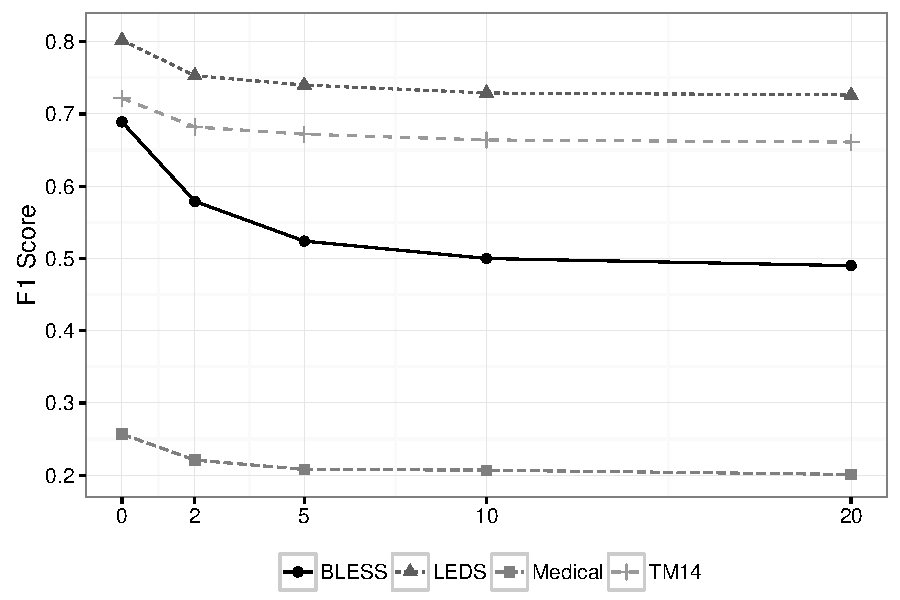
\includegraphics[width=0.45\textwidth]{plots/window}
%  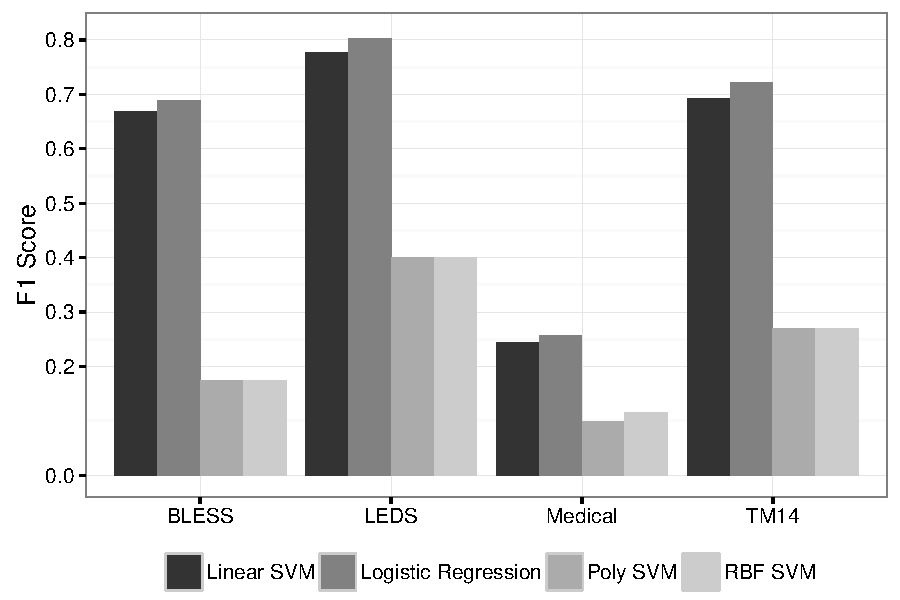
\includegraphics[width=0.45\textwidth]{plots/kernel}
%  \caption{(a) Performance over different BoW context window sizes. 0 indicates a syntactic space.
%           (b) Comparing Logistic Regression with Linear, Polynomial, and RBF SVMs.}
%  \label{fig:hyperparms}
%\end{figure}

\subsubsection{Concerning Lexical Memorization}
\label{sec:lexmem}

Partially motivation for methodology of 

\begin{table}
\begin{center}
  \begin{small}
  \begin{tabular}{|llll|}
    \hline
    LEDS & BLESS & Medical & TM14\\
    \hline
     %% baroni           %% bless             %% levy               %% turney_lemma           \\
     material       &      goods             &     item           &      sensitiveness          \\
     structure      &      lifeform          &     unlockable     &      tactility              \\
     object         & {\bf item}             &     succor         &      palate                 \\
     process        & {\bf equipment}        &     team-up        &      stiffness              \\
     activity       & {\bf herbivore}        &     non-essential  &      content                \\
%     environment    &      omnivore         %&     40px           &      ductility              \\
%     element        & {\bf creature}        %&     crimefighter   &      musculature            \\
%{\bf practice}      &      life-form        %&     material       &      dimensionality         \\
%     nature         & {\bf artifact}        %&     assitance      &      quality                \\
%     organism       & {\bf pest}            %&     nourishment    &      angulation             \\
    \hline
  \end{tabular}
  \end{small}
\end{center}
\caption{Most similar words to the prototype $\hat H$ learned by the Concat model. Bold items
appear in the dataset.}
\label{tab:wordsim}
\end{table}



\begin{table}
\begin{center}
  \begin{small}
  \begin{tabular}{|ll|}
    \hline
    LEDS & BLESS\\
    \hline
      nmod:such\_as+animal             &  nmod:such\_as+submarine           \\
      acl:relcl+identifiable           &  nmod:such\_as+ship                \\
      nmod:of\depinv+determine         &  nmod:such\_as+seal                \\
      nmod:of\depinv+categorisation    &  nmod:such\_as+plane               \\
      compound+many                    &  nmod:such\_as+rack                \\
      %nmod:such\_as+pot                &  nmod:such\_as+rope                \\
      %nmod:such\_as+bone               &  nmod:such\_as+box                 \\
      %nmod:of\depinv+strangeness       &  nmod:such\_as+bat                 \\
      %amod+unassociated                &  nmod:such\_as+pot                 \\
      %compound+similar                 &  nmod:such\_as+container           \\
    \hline
    Medical & TM14\\
    \hline
      nmod:such\_as+patch              &  amod+desire                       \\
      nmod:such\_as+skin               &  amod+heighten                     \\
      nmod:including+skin              &  nsubj\depinv+disparate            \\
      nmod:such\_as+tooth              &  nmod:such\_as+honey               \\
      nmod:such\_as+feather            &  nmod:with\depinv+body             \\
      %nmod:including+finger            &  nsubj\depinv+unconstrained        \\
      %nmod:such\_as+ear                &  compound\depinv+gratification     \\
      %nmod:such\_as+heart              &  compound\depinv+comfort     \\
      %nmod:such\_as+foot               &  nsubj\depinv+composite            \\
      %compound+similar                 &  nmod:such\_as+label               \\
\hline
  \end{tabular}
  \end{small}
\end{center}
\caption{Most similar contexts to the prototype $\hat H$ learned by the Concat model.}
\label{tab:ctxsim}
\end{table}



\begin{table}
\begin{center}
\begin{tabular}{|l|rrrr|}
  \hline
  Model                           &   LEDS   &  BLESS   &   Medical &      TM14  \\
  \hline
  Cosine (Baseline)               &    .789  &    .225  &    .165  &      .674  \\
  \hline
  Concat                          &    .802  &    .689  &    .257  &      .722  \\
  Diff                            &    .809  &    .496  &    .226  &      .672  \\
  Asym \cite{roller:2014:coling}  &    .878  &    .546  &    .227  &      .677  \\
  Ksim \cite{levy:2015:naacl}     &{\bf.912} &    .596  &{   .278} &  {\bf.730} \\
  MProto \cite{roller:2016:emnlp} &    .909  &{\bf.712} &{\bf.295} &      .726  \\
  \hline
\end{tabular}
\end{center}
\caption{Mean F1 scores for each model and dataset.}
\label{tab:results1}
\end{table}

%\begin{figure}
%  \centering
%  \caption{Caption here. Note this graph should probably be redone given the tuning procedure.}
%  \label{fig:kernel}
%\end{figure}






Knowing that the Concat classifier acts primarily as a feature detector, we
ask whether this can be combined with similarity-based insights of models like
Ksim and Cosine. To this end, we propose a novel model which exploits the
Concat classifier, extends its modeling power, and adds two other types of
evidence proposed in the literature: overall similarity, and distributional
inclusion.


The model works through an iterative procedure similar to Principal Component
Analysis (PCA). Each iteration repeatedly trains a Concat classifier under the
assumption that it acts as a feature detector, and then explicitly discards
this information from the distributional vectors. By training a new feature
detector on these modified distributional vectors, we can find additional
features indicative of entailment which were not captured by the first
classifier. This is similar to how in Principal Component Analysis, the
second principal component is computed after the first principal component
has been removed from the data.

The main insight is that after training some feature detector using Concat,
we can {\em remove} this feature from the distributional vectors through
the use of {\em vector projection}.
Formally, the vector projection of $x$ onto
a vector $\hat p$, $\text{proj}_{\hat p}(x)$ finds the {\em component} of $x$
which is in the direction of $\hat p$,
\begin{equation*}
  \text{proj}_{\hat p}(x) = \left(\frac{x^\top\hat p}{\|\hat p\|}\right)\hat p.
\end{equation*}
Figure~\ref{fig:vecproj} gives a geometric illustration of the vector
projection. If $x$ forms the hypotenuse of a right
triangle, $\text{proj}_{\hat p}(x)$ forms a leg of the triangle. This also
gives rise to the {\em vector rejection}, which is the vector forming the third
leg of the triangle. The vector rejection is orthogonal to the projection, and
intuitively, is the original vector after the projection has been removed:
\begin{equation*}
  \text{rej}_{\hat p}(x) = x - \text{proj}_{\hat p}(x).
\end{equation*}

\begin{figure}
  \begin{center}
  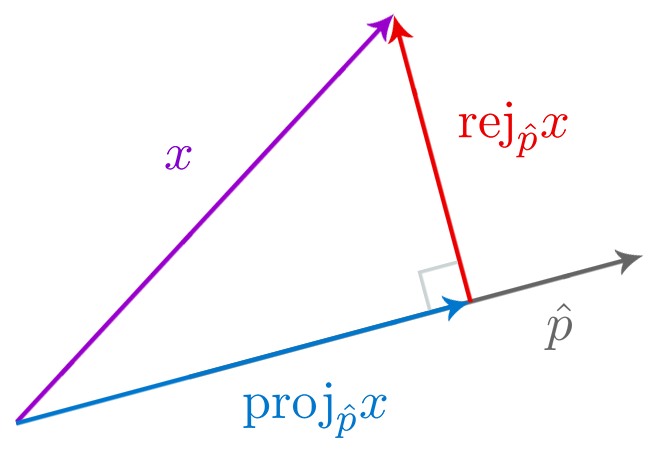
\includegraphics[width=0.30\textwidth]{vecproj}
\end{center}
\caption{A vector $\hat p$ is used to break $H$ into two orthogonal components,
its projection and the rejection over $\hat p$.}
\label{fig:vecproj}
\end{figure}

Using the vector rejection, we take a learned Hearst Pattern detector $\hat p$,
and remove these features from each of the data points. That is, for every data
point $\langle H, w\rangle$, we replace it by its vector rejection and rescale
it to unit magnitude:
\begin{align*}
  H' & = \text{rej}_{\hat p}(H) / \|\text{rej}_{\hat p}(H)\|\\
  w' & = \text{rej}_{\hat p}(w) / \|\text{rej}_{\hat p}(w)\|
\end{align*}
A new classifier trained on the $\langle H', w'\rangle$ data must now learn
a very different decision plane than $\hat p$, as $\hat p$ is no longer present
in any data points. This new classifier must perform strictly worse than the
original, otherwise the first classifier would have learned this hyperplane.
Nonetheless, it will be able to learn {\em new} Hearst patterns which the
original classifier was unable to capture. By repeating this process several
times, we can find several Hearst pattern detectors, $\hat p_1, \ldots, \hat
p_n$.

In each iteration $i$ of the procedure, we generate a four-valued feature vector
$F_i$, based on the Hearst pattern detector $\hat p_i$. Each
feature vector contains (1) the similarity of $H_i$ and $w_i$ (before projection);
(2) the Hearst detector
$\hat p_i$ applied to $H_i$; (3) the Hearst detector $\hat p_i$ applied to $w_i$; and
(4) the difference of 2 and 3.
\begin{align*}
  & F_i(\langle H_i, w_i\rangle, \hat p_i)\\
  & \qquad = \langle H_i^\topw, H_i^\top\hat p_i, w_i^\top\hat p_i, H_i^\top\hat p_i - w_i^\top\hat p_i\rangle
\end{align*}
These four ``meta''-features capture all the benefits of the Hearst pattern
detector (slots 2 and 3), while still addressing Concat's issues with
similarity arguments (slot 1) {\em and} distributional inclusion (slot 4).

The union of all the feature vectors $F_1, \ldots, F_n$ from repeated iteration form a
$4n$-dimensional feature vector which we use as input to another classifier.
This classifier is trained on the exact same training data as each of the
individual Hearst Pattern detectors, so the procedure only acts as a method of
feature extraction. We use an SVM with an RBF-kernel, as we found it to work
best, though several nonlinear classifiers also to do well.

The only free hyperparameter of the model is $n$, the number of iterations of
the PCA-like procedure. We found that performance improves substantially on all
datasets with at least two iterations, but then falls off slowly after five or
more iterations. We chose to use four iterations for all final models.

\subsection{Lexical Substitution (Roller and Erk, 2016a)}
\label{sec:pic}

\begin{figure}
  \centering
  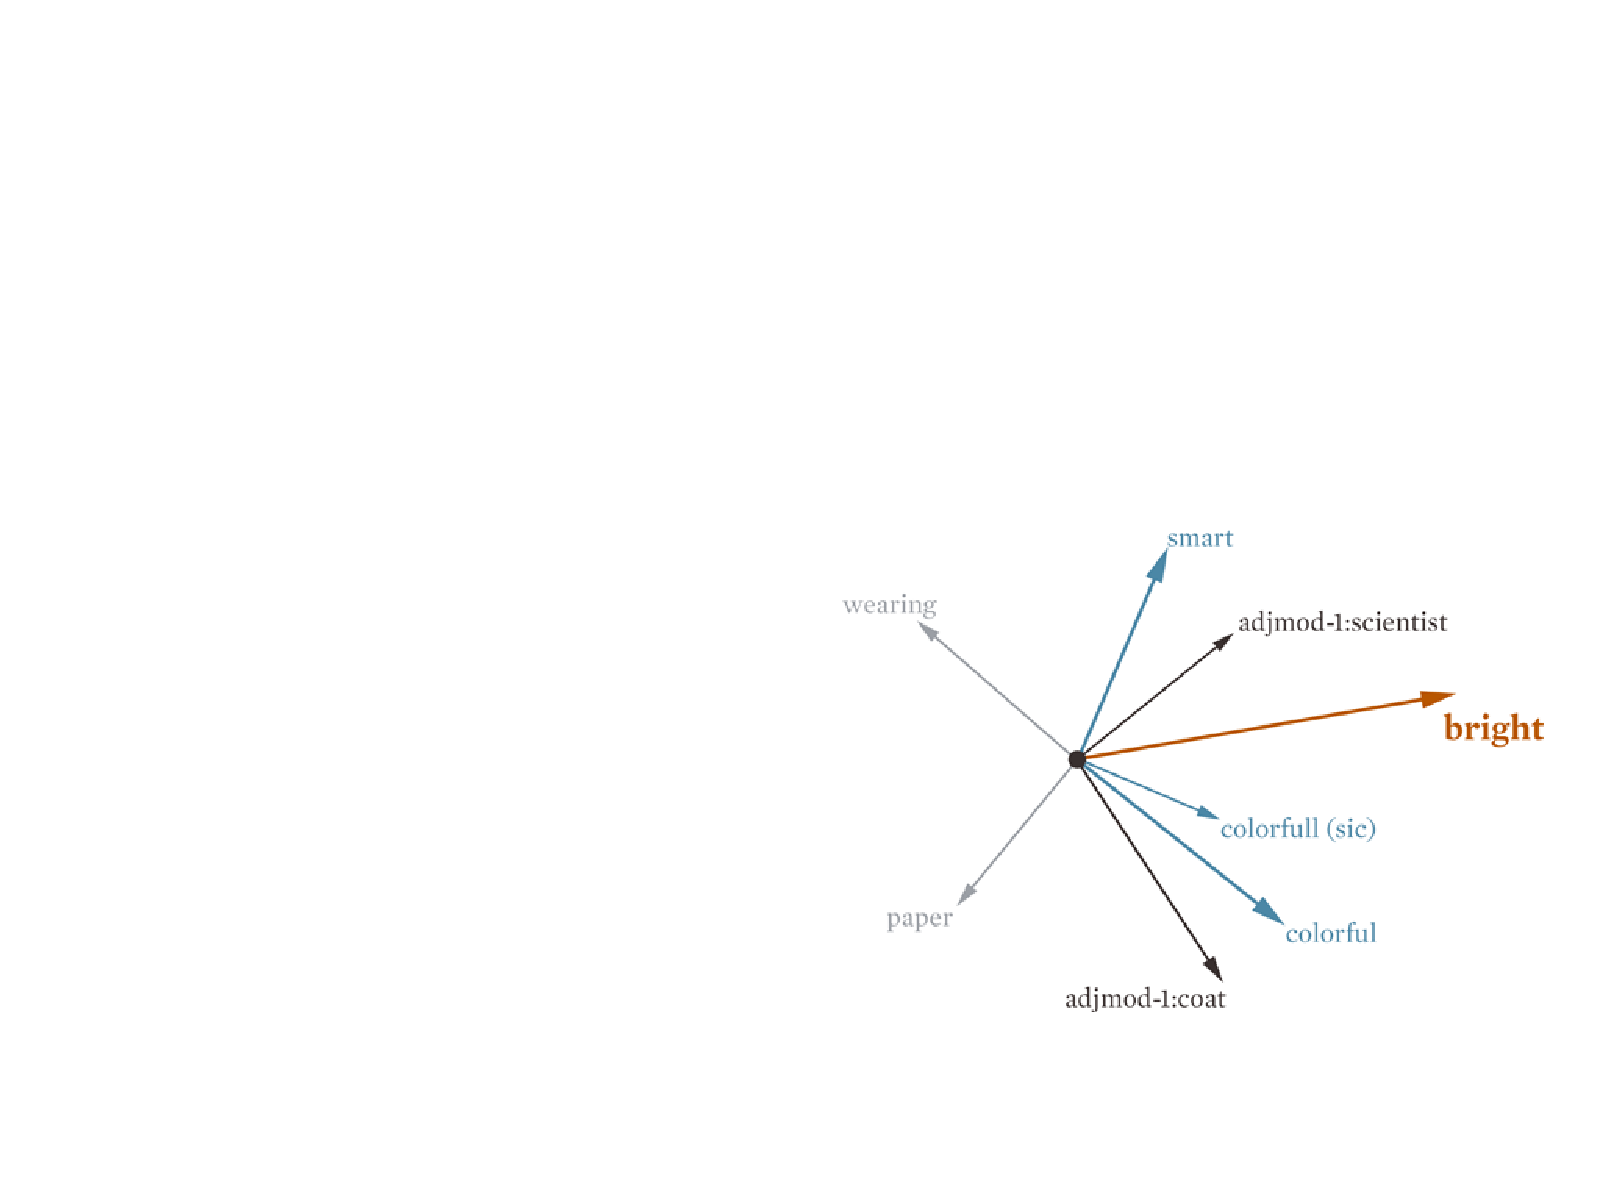
\includegraphics[width=0.75\textwidth]{figures/substitution}
  \caption{Caption here.}
  \label{fig:substitution}
\end{figure}



We propose a new measure, called Probability-in-Context (PIC), based
on SGNS context vectors to estimate the appropriateness
of a lexical substitute. Similar to \balAddCos, the measure has two equally-weighted,
independent components measuring the appropriateness of the substitute
for both the target and the context, each taking the form of a softmax:\footnote{Note that $P(s|t)$ measures paradigmatic similarity
  of $s$ and $t$, while $P(s|C)$ is syntagmatic fit to the
  context.
  %Both take the same shape of a dot product.
  For $P(s|t)$,
  Mikolov et al.~\shortcite{mikolov:2013:iclr} show that cosine
  similarity of SGNS embeddings predicts
  paradigmatic similarity. $P(s|C)$ can be interpreted as the PMI of
  $s$ and $C$~\cite{levy:2014:nips}.}
\begin{equation}
  \begin{aligned}
  \mbox{PIC}(s | t, C) &= P(s | t) \times P(s | C)\\
  P(s | t) &= \frac{1}{Z_t}\exp\left\{s^\top t\right\}\\ %{\sum_{s'}\exp\left\{s'\cdot t\right\}}
  P(s | C) &= \frac{1}{Z_C}\exp\left\{\sum_{c\in C}s^\top\left[Wc + b\right]\right\}
  \end{aligned}
  \label{eqn:pic}
\end{equation}

The values $Z_t$ and $Z_C$ are normalizing constants to make sure each
distribution sums to one. This measure has two free parameters, $W$ and $b$,
which act as a linear transformation over the context vectors. These parameters
are estimated from the {\em original corpus}, and are trained to maximize
the prediction of a {\em target} from only its syntactic contexts (c.f. Section~\ref{sec:training}).
Given this formulation, a natural question is why not train the embeddings to optimize the
softmax directly? We choose to parameterize the measure rather than the
embeddings because (i) SGNS embeddings are already popular and readily
available and
(ii) it ensures the quality of embeddings remains constant across experimental 
settings.

To measure the importance of parameterization, we
also compare to a non-parameterized PIC (\ourmeas), which only uses a softmax over the
dot product:
\begin{equation}
  \begin{aligned}
  \mbox{nPIC}(s | t, C) &= P(s | t) \times P_n(s | C)\\
  P_n(s | C) &= \frac{1}{Z_n}\exp\left\{\sum_{c\in C}s^\top c\right\} %{\sum_{s'}\exp\left\{\sum_{c\in C}{s'\cdot c}\right\}}
  \end{aligned}
  \label{eqn:npic}
\end{equation}



\begin{table}
\begin{center}
\begin{tabular}{|l|r|r|r|}
  \hline
  {\bf Measure} & {\bf SE07} & {\bf Coinco} & {\bf TWSI2}\\
  \hline\hline
  %\multicolumn{4}{|c|}{Candidate Ranking (GAP)}\\
  %\hline
  %\ooc               &     44.2   &     44.5  &     57.9       \\
  %\addCos            &     51.2   &     46.3  &     62.2       \\
  %\balAddCos         &     49.6   &     46.5  &     61.3       \\
  %\hline
  %\ourmeas           &     51.3   &     46.4  &     61.8       \\
  %\ourmeasparam      & {\bf52.4}  & {\bf48.3} & {\bf62.8}      \\
  %\hline\hline
  %\multicolumn{4}{|c|}{All-Words Ranking (Mean Precision@1)}\\
  %\hline
  Out-of-context Baseline                  &     11.7   &    10.9   &      9.8       \\
  addCos                                   &     12.9   &    10.5   &      7.9       \\
  balAddCos                                &     13.4   &    11.8   &      9.8       \\
  \hline
  nPic                                     &     17.3   &    16.3   &     11.1       \\
  PIC                                      & {\bf19.7}  &{\bf18.2}  & {\bf13.7}      \\
  \hline
  %\hline
  %\multicolumn{4}{|c|}{All-Words Ranking (Mean Precision@3)}\\
  %\hline
  %\ooc               &     9.7    &     8.6   &     7.0       \\
  %\addCos            &     9.0    &     7.9   &     6.1       \\
  %\balAddCos         &     9.8    &     9.1   &     7.4       \\
  %\hline
  %\ourmeas           &    13.1    &    12.1   &     7.9       \\
  %\ourmeasparam      &{\bf14.8}   &{\bf13.8}  &{\bf10.1}      \\
  %\hline
\end{tabular}
\end{center}
\caption{Lexical Substitution results for candidate ranking (GAP) and all-words
ranking tasks (P@1, P@3).}
\label{tab:precision}
\end{table}

Table~\ref{tab:precision} contains results for all measures across all
experimental settings.

The first observation we make is that the \ourmeasparam~measure performs best
in all evaluations on all datasets by a significant margin.\footnote{Wilcoxon signed-rank test, $p < 0.01$}
In the GAP evaluation, all measures
perform substantially better than the \ooc~baseline, and the \ourmeas~measure
performs comparably to \balAddCos. We note that context-sensitive
measures give the most improvement in SE07, reflecting its greater emphasis on
polysemy.

As we turn to the all-words ranking evaluations, we observe that the absolute numbers are
much lower, reflecting the increased difficulty of the task. We also see the
that \ourmeas~and \ourmeasparam~both improve greatly over all baselines: The
\ourmeas~measure is a relative 30\% improvement over \balAddCos~in SE07 and
Coinco, and the \ourmeasparam~measure is a relative 50\% improvement over
\balAddCos~in 5 evaluations.

Since both measures have a clear improvement over the baselines, especially in
the more difficult all-words task, we next strive to understand why.

\begin{table*}[t]
  \begin{center}
  \begin{tabular}{|cccc|}
    \hline
    \ooc             & \balAddCos            & \ourmeas         & \ourmeasparam\\
    \hline\hline
    \multicolumn{4}{|c|}{You can sort of challenge them well, did you}\\
    \multicolumn{4}{|c|}{{\bf really} know the time when you said yes?}\\
    \hline
    {    trully              } & {    proably             } & {    realy               } & {\bf actually            } \\
    {\bf actually            } & {    trully              } & {\bf truly               } & {\bf truly               } \\
    {    actaully            } & {    acutally            } & {\bf actually            } & {    already             } \\
    {    acutally            } & {    actaully            } & {    hardly              } & {    barely              } \\
    {    proably             } & {    probaly             } & {\bf definitely          } & {    just                } \\
    \hline
  \end{tabular}
  \end{center}
  \caption{Example where the \ourmeasparam~performs better in the All-Words Ranking task. The target word and correct answers
  are bolded.}
  \label{tab:cherry}
\end{table*}

We first provide a cherry-picked examples to give intuitions about why
our model performs better. Table~\ref{tab:cherry} contains the cherry example,
where our model performs better than prior work. While OOC
and \balAddCos~both suggest replacements with reasonable semantics, but are
all misspelled. \ourmeas~and \ourmeasparam~only pick words with the correct spellings,
with the exception of ``realy.''

We consider a few experiments with this hypothesis that the measures do better
because they capture better {\em unigram} statistics than the baselines. Recent literature found that the vector
norm of SGNS embeddings correlates strongly with word frequency
\cite{wilson:2015:arxiv}. We verified this for ourselves, computing the Spearman's
rank correlation between the corpus unigram frequency and the vector length
and found $rho = 0.90$, indicating the two correlate very strongly. Since the
dot product is also the unnormalized cosine, it follows that \ourmeas~and
\ourmeasparam~should depend on unigram frequency.

To verify that the \ourmeas~and \ourmeasparam~measures are indeed preferring more frequent
substitutes, we compare the single best predictions (P@1) of the \balAddCos~and
\ourmeas~systems on all-words prediction on Coinco. Roughly 42\% of the predictions made
by the systems are identical, but of the remaining items, 74\% of
predictions made by \ourmeas~have a higher corpus frequency than \balAddCos~(where
chance is 50\%). We find \balAddCos~and \ourmeasparam~
make the same prediction 37\% of the time, and \ourmeasparam~predicts a
more frequent word in 83\% of remaining items. The results for SE07 and
TWSI2 are similar.

This indicates that the unigram bias is even higher for \ourmeasparam~than
\ourmeas. To gain more insight, we manually inspect the learned parameters $W$
and $b$. We find that the $W$ matrix is nearly diagonal, with the values along
the diagonal normally distributed around $\mu=1.11$ ($\sigma=0.02$) and the rest
of the matrix normally distributed roughly around 0 ($\mu$=2e-5, $\sigma$=0.02). This
is to say, the \ourmeasparam~model is approximately learning to {\em exaggerate} the
magnitude of the dot product, $s^\top c$. This suggests one could even replace our
parameter $W$ with a single scaling parameter, though we leave this
for future work.

To inspect the bias $b$, we compute the inner product of the $b$ vector with
the word embedding matrix, to find each word's a priori bias, and correlate it with word frequencies. We find
$rho=0.25$, indicating that $b$ is also capturing unigram
statistics.

Is it helpful in lexical substitution to prefer more frequent substitutes? To
test this, we pool all annotator responses for all contexts in Coinco, and find
the number of times a substitute is given correlates strongly with frequency
($rho=0.54$).

These results emphasize the importance of incorporating unigram
frequencies when attempting the lexical substitution task (as with
many other tasks in NLP). Compared to
cosine, the dot product in \ourmeas~stresses unigram frequency, and
the parameters $W$ and $b$ strengthen this tendency.
%  (as with so many
% other tasks in NLP). Such a result may seem obvious in retrospect, but many
% prior works in Lexical Substitution simply do not take this into account.

\section{Proposed Work}

We now describe the general proposed methods of further research. The proposed
future work breaks into two broad categories: short-term proposals,
which must be completed for the final thesis, and long-term proposals, which
are more ambitious research directions that may take much longer to successfully
pursue.

The proposed short term work focuses predominantly on how the more recent
successful research may contribute to a larger RTE system: While the completed
work has shown successful results on the two tasks of Lexical Entailment and
Lexical Substitution, these newer models have not yet been applied to the end
goal of Textual Entailment. We propose multiple methods to test our models
in an end-to-end RTE system.

The long term work follows from three broad directions forward: (1) encouraging
taxonomic consistency of predictions in Lexical Entailment; (2) better integration
of a wider context into the Lexical Substitution system; and (3) a more sophisticated
distributional model which reuses information when possible.

\subsection{Short Term Proposals}

In this section, we propose and discuss several additional experiments which
should be completed for the final thesis. We break the section into experiments
for Lexical Entailment, and experiments for Lexical Substitution. All are
proposed primarily with integration into a final RTE subsystem in mind.

\subsubsection{Lexical Entailment}

\paragraph{H-features for non-Hypernymy Relations}

In Section~\ref{sec:hfeatures}, we discussed how the H-Features model
is able to exploit multiple H-feature detectors in order to improve the results
and modeling power of a hypernymy detection system. Indeed the H-features
model outperformed the Asym and Ksim models when evaluated on the same metric of
F1-score in hypernymy prediction.

However, there exist many relations {\em other} than hypernymy are useful to
distinguish in textual entailment: for example, we saw in
Section~\ref{sec:rtesubsystem} that cosine similarity is indicative of entailment
at moderate levels, where it reflects general similarity, but {\em counter-indicative}
of entailment at very high levels, where it is most indicative of co-hyponymy.
Indeed, dividing word relationships into hypernymy and non-hypernymy could be
viewed as dividing the world into living and nonliving things: while this is
a very important distinguishing feature, it may be helpful to identify a bit more
information.

Indeed, the results shown in Table~\ref{tab:bless-and-entailment-v-space} show
the accuracy of the Asym and Baroni classifiers on a four-way relationship
prediction task: hypernymy, cohyponymy, meronomy, and random, yet the
experiments in Section~\ref{sec:hfeatures} only describe performance in a
binary hypernymy-or-not classification task. We propose the H-features
model of Section~\ref{sec:hfeatures} be extended and evaluated on its
performance in other relationships.

There are several ways that the model could be extended. The one we believe
will be most successful is one that trains several binary H-features models:
one for hypernymy-vs-nonhypernymy, one for meronomy-vs-nonhypernymy, etc.
Similar to how the PCA procedure was used only as a form of feature-extraction
for the final prediction, each of the binary classifier iterations will be also
used for feature extraction for a final classifier.
That is, we will use the procedure described in Section~\ref{sec:hfeatures}
to extract several iterations of features for hypernymy, then completely repeat
the procedure for meronomy and co-hyponymy. The resulting features from each
of the classifiers will be concatenated for a final four-way classifier prediction.
Another alternative would be to try to learn the four-way classifiers concurrently
(e.g., a softmax instead of logistic regression), and extract the corresponding
H-features at this level.

There are interesting research questions that stem from this procedure, beyond
just final performance scores. One is what distributional-level features will
be learned as prototypical of meronyms, or co-hyponyms? As we saw in
Table~\ref{tab:ctxsim}, the classifier automatically learned to pick
out well-known Hearst patterns, indicative of hypernymy. It remains to be seen
whether it will pick out additional Hearst patterns indicative of other
relations: for example, simple conjunctions for co-hyponymy (e.g., {\em cats
and dogs}) or the possessive for meronomy (e.g., {\em cat's tail}).

\paragraph{H-features Model for RTE}

The results of Section~\ref{sec:rtesubsystem} showed that the Asym hypernymy
prediction model can provide strong improvements in a complete, end-to-end RTE
system, especially when combined with traditionally hand-engineered features.
Yet, as we also saw in Section~\ref{sec:hfeatures}, the H-features
model allows for greater modeling power and significant improvements on multiple
lexical entailment systems. Yet we do not yet know how much the H-features
model is able to contribute as one part of the larger RTE pipeline.

We suspect, given its substantial improvements over Asym in lexical datasets,
that it will also be able to be able to improve the full system. However, it
remamins unclear what is the best way to integrate it with additional
hand-engineered features used in the RTE system.  One possibility would be to
simply use the H-features's feature extraction procedure to provide
additional information to the lexical entailment classifier. Yet the classifier
used in Section~\ref{sec:rtesubsystem} was a linear classifier over the hand
engineered features, which outperformed nonlinear versions. Unfortunately, we
found in Section~\ref{sec:hfeatures} that the final ensemble classifier
{\em must} be nonlinear, else it does not gain any additional power in the
repeated iterations. Resolving this conflict may be difficult, though we
suspect it may be alleviated by more careful hyperparameter tuning of nonlinear
models.

These proposed experiments will also need to be tightly coupled with the
complete non-hypernymy detector discussed in the previous section. If H-features
are useful useful for predicting co-hyponymy or meronomy, it also stands to
reason that they should be useful in the final RTE subsystem. We will need to
explore the best form of combination with both kept in mind.

\subsubsection{Lexical Substitution in RTE}

In Section~\ref{sec:lexsub}, we argued that Lexical Substitution is strongly
related to the tasks of lexical and textual entailment, partially standing
as a form of context-specific synonym detection. Unfortunately, we have
yet to provide any results indicating that Lexical Substitution may actually
contribute to the complete RTE system.

We propose that the Lexical Substitution model described in
Section~\ref{sec:pic} be used to provide additional information to
the Lexical Entailment classifier used in Section~\ref{sec:rtesubsystem}.

There are at least two possibilities for how a Lexical Substitution model could
contribute to the task. The first, and one we believe most likely to be
helpful, is to simply add the context-similarity features of the Lexical
Substitution model as another feature in the Lexical Entailment classifier.
That is, for a pair of words in the SICK dataset, measure the similarity of
their contexts using the $P(s|C)$ or $P_n(s|C)$ values proposed in
Equations~\ref{eqn:pic}~and~\ref{eqn:npic}. This could possibly help
with some tricky cases where two senses of a word could lead to different conclusions.
For example, ``EXAMPLE HERE.''

It may also be necessary to use a similar trick to the cosine binning technique
described in Section~\ref{sec:rtesubsystem}: it could be that different levels
of contextual similarity give different indications as to entailment, especially
given the close relationship between our Lexical Substitution model and
cosine similarity. Variations on this trick may also be necessary to test:
since our Lexical Substitution model gives a score over the entire vocabulary,
the binning may need to be logarithmic, or measured as a percent of vocabulary
which is a better substitute than the queried consequent.

The second possibility for how Lexical Substitution could contribute is in
the {\em alignment} preprocessing procedure: while we currently only choose
which word pairs to align with our greedy cosine-similarity based method, it
could be that the $P(s|C)$ model provides additional information to make
smarter alignments. For example, we each token in the antecedent, we could
align it with the consequent's token that acts as the best lexical substitute
{\em in-context}, rather than the out-of-context measure we presently use.

Ultimately though, we suspect improvements to RTE from either proposed
application of the Lexical Substitution model may be marginal, or even
negative, as polysemy is not common in the RTE dataset that we use. We may
need to manually identify which RTE pairs exhibit polysemy the strongest, or
manually construct a small dataset of sentences with polysemy in order to
show positive results.

\subsection{Long Term Proposals}

We now describe some possible longer term research questions which could be
addressed in the final thesis. Success in any of these items would
be significant contributions to the field, and are therefore more ambitious and
risky than the short-term proposals.

\subsubsection{Taxonomic Consistency in Hypernymy Prediction}

Presently in our hypernymy-prediction models, relationships between all
pairs of words are made independently: the prediction of whether ``cat is an
animal'' has no bearing on whether ``dog is an animal'', aside from their
distributional similarity. While this is a straightforward application of
machine learning principles to the problem, it ignores one important fact: that
hypernymy is just one aspect of a complete, well-structured ontology or
taxonomy. Yet, since we predict each word pair individually, there is no
guarantee the final output of the system over all pairs will also be
well-structured.

For example, a hypernymy prediction model could predict that both ``animal is a
hypernym of dog'' and that ``dog is a hypernym of animal'', is though we know
hypernymy is non-reflexive; or it could predict that ``a golden retriever is a
dog'' and ``dog is an animal'' but incorrectly predict that ``gold retriever is
{\em not} an animal,'' violating the transitive property of hypernymy. These
properties of hypernymy are inherent to how it is defined, and our models
should be take this into account.

With this in mind, is it possible to modify our model such that taxonomic
consistency of the output is guaranteed, or at least more consistent? One
possibility would be to use the {\em confidence scores} associated with the
hypernymy predictions, and simply revise the least-confident predictions to
be consistent in a post-processing step. For example, in our reflexive example
above, the more confident of the two predictions will be assumed to be
the correct one.

This idea would likely even benefit further from our short-term proposal to
see how well the H-features model does at predicting relations other
than hypernymy: for example, if we are highly confident that two words are
co-hyponyms, then we can become more confident that they share the same
hypernyms, and vice versa.

This idea of enforcing taxonomic consistency is not new: it was previously
explored by \newcite{caraballo:1999:acl}, who use a clustering algorithm in
order to find co-hyponym terms, and then predict their hypernym using entire
clusters. It was also examined some in \newcite{snow:2004:nips}, who used
syntactic Hearst Patterns to make predictions about hypernymy, and then
linearly interpolated the probabilities of predictions in order to better
conform to these hard taxonomic constraints. Later, \newcite{snow:2006:acl}
proposed a probabilistic model over {\em taxonomies}, allowing them to propose
an algorithm for searching over entire taxonomies constrained by rules about
the transitivity of hypernymy, and reflexivity of co-hyponymy. This taxonomy
search is then used in order to find the single taxonomy which has maximal
probability according to the evidence provided by Hearst patterns, while also
not violating any of the hard constraints.

Although \newcite{snow:2006:acl} found their taxonomy searching algorithm
highly successful with the use of the lexico-syntactic patterns indicative
of hypernymy, such an approach is yet to be tried on classifiers which make
use of distributional information about words. Therefore, the most reasonable
first course of action would to reimplement and examine whether their model
is compatible with the distributional models of hypernymy prediction. On one
hand, it could help tremendously; on the other hand, their model supports only
two forms of constraints (transitivity of hypernymy and reflexivity of
co-hyponyms), leaving open questions about how other constraints should be
imposed.

Another possibility is through the use of the same technology powering the
end-to-end RTE system of \newcite{beltagy:2016:cl}: Markov Logic Networks
(MLNs).  Markov Logic Networks provide a framework for doing probabilistic
logical inference over sets of weighted atoms and logical rules. MLNs are given
a set of weighted First Order Logic (FOL) rules and a database of atoms, and
give reweighted predictions about the probabilities of atoms based on their
consistency with the logical rules. MLNs can encode many
different relations as rules, and perform joint updating of all lexical
relationship predictions.  For example, the rules for transitivity and reflexivity
discussed in \newcite{snow:2006:acl} could be encoded as:
\begin{align*}
  \forall x,y,z. &~\text{hyper}(x,y) \wedge \text{hyper}(y, z) \rightarrow \text{hyper}(x, z),\\
  \forall x,y. &~\text{cohyp}(x,y) \leftrightarrow \text{cohyp}(y,x),
\end{align*}
but other rules, such that co-hyponyms share a hypernym, may also be encoded:
\begin{align*}
  \forall x,y,z. &~\text{cohyp}(x,y) \wedge \text{hyper}(x,z) \rightarrow \text{hyper}(y,z).
\end{align*}

MLNs ability to incorporate {\em weighted rules} would also give room for
flexibility in constraint importance, and allow for {\em some} violations of
constraints when the evidence is simply overwhelming. Therefore, we believe
both the model of \newcite{snow:2006:acl} and an MLN-based model to be strong
candidates for improving lexical relationship prediction by enforcing taxonomic
consistency.

\subsubsection{Sophisticated Contexts for Lexical Substitution}

\paragraph{Wider Contexts in Lexical Substitution}
In the model of Lexical Substitution discussed in Section~\ref{sec:pic}, we
showed how the syntactic neighbors of a target word are useful in predicting
what are the lexical substitutes, or in-context synonyms, of the target word.
Although the syntactic neighbors can indeed capture some kinds of {\em long-distance
dependencies}, there is much greater deal of context available which is
presently not used by the model: namely, the {\em entire rest of the sentence}.

Consider, for example, if the model were able to asked to find the best verb
to fill-in-the-blank in the following two simple sentences:

\begin{center}
  {\em The dog \_\_\_ the tennis ball.}\\
  {\em The dog \_\_\_ the meat ball.}
\end{center}

In both cases, the model will be given the exact same context for the missing
verb: its subject should be {\em dog} and its object should be {\em ball}. However,
humans know that the dog is more likely to {\em chase} or {\em fetch} the tennis
ball, while it is more likely to {\em eat} the meat ball. Without being provided
the additional information about the ball, the model has absolutely no way
to distinguish these two cases. How can this information be integrated into the
model?

Even beyond this simple example, it's already clear from prior work that
additional context can be very useful in the task.
\newcite{vandecruys:2011:emnlp}, for example, proposed model which combined
a syntactic distributional space with a bag-of-words distributional space with
a very large window by finding a shared latent representation of both spaces,
showing modest improvements over each individual space. Furthermore,
\newcite{kawakami:2016:iclr} obtained state-of-the-art results on Lexical
Substitution using a neural network language model which encodes the {\em
entire sentence} as input, though their model also depends heavily on the use
of machine translation data as a sort of proxy for Word Sense Disambiguation
information. Nonetheless, it is clear that there is more useful information
available than our own Lexical Substitution model is allotted.

There two distinct ways we could implement wider contexts into our Lexical
Substitution model: using linguistic knowledge, and using neural networks.
In the former, we could simply use existing linguistic knowledge in order to
model additional syntactic patterns from large corpora. That is, in
addition to modeling the direct neighbors of words which constructing our
distributional space, we could also add pattern-based rules for modeling
indirect neighbors. For example, we could introduce an additional context
in our distributional space for {\tt dobj+compound+\_+meat}; that is, an
additional column for which the direct object of a verb is compounded with
``meat'', and so on for other nouns. Indeed, since our model uses collapsed
prepositional phrases, this is already partially implemented (e.g., we already
model ``to the store'' as {\tt prep:to\_store} rather than just {\tt prep:to}).

A variation of this approach was discussed in \newcite{pado:2007:cl}, the
original proposal of syntactic distributional spaces. In their model, they also
extracted contexts for dependency chains two and three hops away from the
target word, rather than the only the direct neighbors. Since then, most models
have focused mostly on direct neighbors (except for prepositional phrases), as
this approach introduces many additional contexts, making the model
significantly more complex and memory intensive, while also dramatically
increasing the sparsity of the data: the vast majority of 3-hop syntactic
patterns will occur only once in corpus. Indeed, if we use this linguistic
approach, these issues of scaling and sparsity will plague our model as well.

The other possibility for this problem would be to employ modern neural network
models, like the Long Short Term Memory (LSTM) model \cite{hochreiter:1997:nc}.
The LSTM model has become extremely popular in the field of Natural Language
Processing, thanks to recent advances in network initialization
\cite{glorot:2010:aistats}, training techniques
\cite{duchi:2011:jmlr,kingma:2014:arxiv}, and hardware like Graphics Processing
Units (GPUs). Indeed, LSTMs are the basis for the successful model of
\newcite{kawakami:2016:iclr} mentioned previously. LSTMs are a form of a
Recurrent Neural Network, which takes as input a variable-length sequence of
items (tokens), and make some prediction. They have been successfully applied
countless areas of NLP, including language modeling
\cite{sundermeyer:2012:lstm,jozefowicz:2016:arxiv}, sentiment analysis
\cite{kumar:2015:arxiv}, machine translation \cite{sutskever:2014:nips},
textual entailment \cite{bowman:2015:emnlp}, question answering
\cite{hermann:2015:nips}, and recently even lexical entailment
\cite{shwartz:2016:acl}.

More concretely, we could integrate wider syntax using an approach similar to
that of \newcite{shwartz:2016:acl}. In their model, a syntactic chains
connecting two target words was used to classify whether the words stand in a
hypernymy relationship or not, acting as a modern neural-network version of
\newcite{snow:2004:nips}. We propose using similar syntactic chains to simply
predict the {\em last word} in the chain, performing the operation for billions
of syntactic chains extracted from large corpora. This model would have the
capability of capturing and remembering relevant long-distance information
whenever it is helpful in predicting the final word. The greatest challenge
in applying this model is scaling it, as LSTM models can take days or weeks
to train when their final output is a prediction over the entire vocabulary.

\paragraph{Joint Models of Syntactic Neighbors}

Another issue with the lexical substitution model discussed in Section~\ref{sec:pic}
is that the model fundamentally assumes independence between each of the syntactic
neighbors. Ultimately, the model suggests substitutes in the above examples by
asking, ``What does a dog do? What is done to a ball? What is the intersection
of these two sets?'' That it uses the unnormalized inner products in Equation~\ref{eqn:pic}
means that one of these questions may be given more weight than another, but they
are still considered independently: the question is never ``What does a dog do
to a ball?''

It is worth considering whether this independence assumption can be relaxed
in some way. Intuitively, it seems obvious that a joint model should be helpful.
Yet, one major issue is that the number of syntactic neighbors is variable:
consider that a verb may have attachments may have only one attachment (intransitive),
two attachments (transitive), or more (ditransitive, prepositional phrase attachments,
adverbs, etc). Similarly, nouns can also stand in many syntactic relations
simultaneously (compound, adjective, prepositional phrase, verb relation, and
others). Since the number of attachments is variable, it's difficult to define
a coherent probabilistic model which does not demand at least {\em some}
independence assumptions. Even if we were to define the model over all possible
syntactic relations for every word, the issue would not be solved: consider
a ``small, furry, brown mouse,'' which has three modifiers all standing
in the {\tt adjmod} relation.

Even if we could define such a model, it would likely be plagued the typical
extreme sparsity issues: for many sentences in our dataset, an {\em exact}
combination of attachments seen is unlikely to appear anywhere, even in
extremely large corpora. Therefore, a naive joint model is likely to estimate
the probability as zero for most everything.

As with the proposed methods for including wider contexts, we could potentially
address these issues using either linguistic knowledge, or neural networks.  To
address the concerns using linguistic knowledge, we could again mark certain
rules should be modeled jointly, and assume independence between the remaining
syntactic relations. For example, we could model transitive verbs jointly, but
assume independence from adverbs and prepositional modifiers; or we could
jointly model two adjective modifiers, but assume independence once we
encounter three or more. Again, rules similar to the ones discussed in
\newcite{pado:2007:cl} would be a good starting point, and others could be
proposed in qualitative analysis of the data.

The other possibility is to use LSTMs in order to jointly model the different
modifiers. Since LSTMs are able to handle a variable-length sequence as input,
they seem to be a good candidate for creating a joint model over all the
attachments in a principled manner. Unfortunately, LSTMs also assume that the
{\em order} of the sequence is important, which is not the case for our problem:
there is no inherent ordering of syntactic attachments. We could canonicalize
the ordering (simply insisting that, for example, subjects are always presented
before objects), but it remains unclear whether this is useful. We could also
{\em randomize} the order the attachments are presented: since there are many
permutations, this could substantially increase the amount of training data
available, since each sentence could then generate many training examples: one
where subject is first, one where object is first, etc. However, preliminary
experiments showed difficulty with this second approach: the $PIC$ model came
about when our first attempts at using LSTMs were unsuccessful.

Nonetheless, it is encouraging that the same linguistic and neural network
approaches could be potentially useful for both introducing wider context,
and joint modeling.

\subsubsection{Generalized Distributional Spaces for Entailment and Substitution}

Our final long term proposal is fairly different from the other two: while
those were ideas to directly impact performance on the two tasks we have
since focused our attention, our last idea focuses more broadly on how
we can improve distributional spaces altogether.

We begin with an observation about the process described in
Section~\ref{sec:dist} when constructing a syntactic distributional space.
When constructing a distributional space, the final step involves finding a
matrix factorization for the extremely large, extremely sparse word-context
co-occurrence matrix. In syntactic spaces, the contexts are distinguished by
the neighboring word {\em together} with its syntactic relation. That is there
is one context for {\tt nsubj\_dog} and another for {\tt dobj\_dog}. This is a
powerful notion, and one that gives the syntactic spaces their ability
to model selectional preferences: without distinguishing these relations,
the model would be much like to the bag-of-words spaces.

Yet, modeling each of these contexts independently also seems to be wasting
a large amount of information: that it is the same lexical item being modified
by two different syntactic relations. If this information is ignored, then
we must assume we have excellent corpus statistics for how every word stands
in every relation. Yet this rarely happens, and one of the important
steps in constructing a syntactic distributional space is to limit modeling
to only the top one million most frequent contexts, where the statistics are
still plentiful enough for modeling. But in defining a cutoff at all, we
are also ignoring a lot of information: by Zipf's law, half of the data
is in the long tail. Do we really want to throw away all this data?

We ask then, to what degree can the {\em syntactic relations} be separated
from the {\em words} in syntactic distributional spaces? 
Can these context vectors we rely heavily on in our work be {\em generatively
modeled}? Perhaps one way to approach this would be to model it as a
composition function:
\begin{equation*}
  \vec{ {\tt nsubj\_dog} } = f({\tt nsubj}, \vec{dog})
\end{equation*}
In this view, we would need to learn one function, $f$, which took in a syntactic
relation and a dog, and produced a {\em context vector} on how dog acts in the
subject position. One possibility would be to use vector concatenation,
treating the relation and the word as separate components, independent of each
other. Intuitively, this does not seem to capture the the essence of our
proposal, but it could act as a baseline model:
\begin{equation*}
  \vec{ {\tt nsubj\_dog} } = \langle \vec{dog} ; \vec{nsubj} \rangle
\end{equation*}

Another possibility would be to treat the procedure as a form of post-processing
generalization. For example, we could learn the context vectors as we do now, and
then attempt to learn to predict the observed context vectors from the input
components. For example, perhaps after performing the concatenation, a simple
linear regression could combine them:
\begin{equation*}
  \vec{ {\tt nsubj\_dog} } = W\langle \vec{dog} ; \vec{nsubj} \rangle + \vec{b}
\end{equation*}
This is a relatively weak model, but it would still enable us to predict
information about novel combinations of syntactic relations and words. The
model could be even more sophisticated, being a neural network instead; however,
neural networks are known to be easier to train for classification than
regression \cite{needcite}.

Another variation of this linear regression idea, would be to model each
syntactic relation as a function {\em applied} to the vector. For example,
we would learn a separate $W$ for {\tt nsubj}, {\tt dobj}, etc:
\begin{equation*}
  \vec{ {\tt nsubj\_dog} } = W_{{\tt nsubj}}\vec{dog}
\end{equation*}
This gives the model many more free parameters, but may present some difficulty
for the rarest syntactic relations, where there could easily be more parameters
in $W$ than examples, though perhaps heavy regularization of $W$, or even
constraining it to be diagonal could be beneficial. Modeling the behavior in
this way would draw greater parallels to other areas of the literature,
like compositional distributional semantics \cite{baroni:2010:emnlp,coecke:2011:la,grefenstette:2011:emnlp,baroni:2014:li}, the
bilinear models proposed in GloVe \cite{pennington:2014:emnlp}, and the recursive
composition models for sentiment analysis \cite{socher:2013:emnlp}.

Alternatively, we could  try to learn the distributional vectors from scratch
using a similar model. Recall that the dimensionality reduction procedure
simply tries to predict the Pointwise Mutual Information between a word and
a context. Rather than performing the dimensionality reduction, then regression,
we could encode our generative principals into the dimensionality reduction.
In this way, a successful model may look something more like {\em tensor
factorization}. For example, we could model the PMI between a word ($v$),
and a relation-context pair ($r, c$) as:
\begin{equation*}
  PMI(v, r, c) = {\bf v}^\top {\bf W}_{r} {\bf c},
\end{equation*}
where ${\bf W_r}$ is a matrix. This is essentially the same as the linear
regression model proposed in the above paragraph, but performed at a different
step. Unfortunately, tensor factorization is generally very difficult
\cite{haastad:1990:ja,hillar:2013:jacm}, and there is no such convenient canonical factorization for
tensors, as the SVD is for matrices, though Tucker Decomposition
is one well-studied approach \cite{tucker:1966:psy}. Finding the ideal
factorization is likely to be a very difficult optimization problem without
major simplifying assumptions, and one beyond our own expertise.

However, an excellent place to start would be in the Information Extraction
literature, especially those focused on Statistical Relational Learning. These
works seek to find generative representations for (subject, verb, object)
triples, like {\tt IBornIn(John, Athens)}, and there is a rich literature
regarding approaches to this very difficult problem.
The approach of \newcite{nickel:2011:icml} is closest to the model we actually
proposed above, but since there has been significant advances in both time
and space complexity
\cite{socher:2013:nips,riedel:2013:naacl,yang:2014:iclr,kuleshov:2015:aistats,trouillon:2016:icml}.

Regardless, if we assume that we {\em can} find any model which successfully
predicts context vectors in a generative manner, then it could lead to
substantial improvements on both tasks of Lexical Entailment {\em and} Lexical
Substitution. For example, we saw in Table~\ref{tab:ctxsim} that certain
syntactic relations are indicative of hypernymy. Therefore, being able to plug
in any two words to and estimate the liklihood that they will stand in this
syntactic relation, like {\tt nmod:such\_as}. Ideally, this should work even
better than directly searching a large corpus to see if the two words are
actually {\em observed} in relation, since the model would assume that similar
words will stand in similar relations.

The problem would also contribute even more greatly to the Lexical Substitution
model we presented. For many examples in our dataset, our model does not have
any context vector representation for one or more of the syntactic neighbors
observed. In a preliminary examination, we found that some X\% of the CoInCo
dataset contain at least one context which not available in our vector space.
The ability to {\em generate} representations for these contexts would be
a simple way to provide the model with more disambiguating information, which
should help in the end task.

Indeed, as we described above, a novel model could easily have larger
implications in other areas of Natural Language Processing, and is therefore
probably the most ambitious and difficult of our long term proposals.

\section{Conclusion}

Distributional Semantics has come a long way in its ability to contribute to
difficult Natural Language Processing tasks. In this proposal, we several
methods for distilling {\em lexical knowledge} out of distributional vectors.
We discussed two models of hypernymy detection, which take as input pairs of
words, and predict whether those models stand in a hypernymy relation.  Through
detailed analysis, we have a clear picture of how these models work, and how
they relate to some of the linguistic literature on Lexical Entailment, like
the Distributional Inclusion Hypothesis and Hearst Patterns. We also saw that
at least one of these models is able to positively contribute to an RTE Lexical
Entailment classifier, which uses a wide variety of lexical cues and resources,
like WordNet and distributional similarity, in order to improve performance in
an end-to-end RTE system. We also discussed a new model of Lexical
Substitution, which we argue is related to lexical entailment by acting as a
form of {\em in-context synonym prediction}. Our Lexical Substitution model
outperforms some comparable baselines, and analysis shows its improvements
derive predominantly from exploiting simple unigram priors.

We also discussed multiple directions for how our work could be extended
in the future. In the short term, we focus on exploring how our H-features
model could also contribute to the RTE Lexical Entailment classifier, and
whether the H-features model is able to model relations other than hypernymy.
We also discussed several ways in which the Lexical Substitution model could
contribute to the RTE Lexical Entailment Classifier. Progress in these areas
would contribute significantly to our thesis that our models extract useful
lexical information for Recognizing Textual Entailment.

Finally, we discussed different long-term directions for future research. These
ideas are much larger, and less guaranteed than the short-term research
proposals, but also reflect our opinion on where the field should go from here.
Namely, we considered how Hypernymy and Relationship prediction could be
improved by imposing simple constraints inherent to ontologies. We also
discussed several ways in which more context could be exploited in Lexical
Substitution, or how we could remove some of the independence assumptions made
by our current model: we note that improvements could easily come by either
exploiting linguistic knowledge about how different syntactic relations
interact, or by using very successful neural network technologies. Lastly, we
considered how current syntactic distributional spaces make an inefficient use
of the available information, and discussed ways they could be extended to be
{\em generative} over syntactic relations, instead of just artificially
limiting the statistics they model. Improvements in these spaces would likely
improve performance of distributional models in many tasks, including
Lexical Entailment and Lexical Substitution.

\pagebreak
\bibliographystyle{aclcite}
\bibliography{refs}

\end{document}
